\documentclass[12pt]{article}
\usepackage[left=1.15in, right=1.15in, top=1in, bottom=1.5in]{geometry}
\usepackage{natbib}
\usepackage{verbatim}
\usepackage{setspace}
\usepackage{booktabs}
\usepackage{caption}
\usepackage{graphicx}
\usepackage{subcaption}
\bibpunct[: ]{(}{)}{;}{a}{}{,} 
\usepackage{authblk}
\renewcommand\Authfont{\normalsize}
\renewcommand\Affilfont{\footnotesize}

\begin{document}
\title{The Forward March of Categorical Tolerance in the United States\thanks{Reserved for acknowledgments}}
\author[1]{Omar Lizardo\thanks{olizardo@soc.ucla.edu}}
\affil[1]{Department of Sociology, UCLA}

\renewcommand\Authands{ and }

\date{\normalsize \today}	
\maketitle

\newpage
\begin{abstract}
\end{abstract}
\newpage
\section*{Introduction}
In a paper published almost a decade ago, \citet{lizardo2016end-4fb}---hereafter L\&S---introduced the idea of \textit{categorical tolerance} to refer to the phenomenon of a growing proportion of the population who refuse to report dislikes of \textit{any} cultural genres---typically musical genres---in a standard social science survey design to measure patterns of cultural taste. In that paper, L\&S noted that categorical tolerance appeared to be on the rise in the United States, going from about five percent of the population in the classic 1993 General Social Survey culture module to about sixteen percent in a then-recent survey of a representative sample of Americans collected in 2012, which matched the GSS 1993 battery of items on likes and dislikes of musical tastes across eighten genres. This resulted in a significant shift in the shape of the univariate count distributions of number of dislikes, which went from a standard Poisson distribution in the GSS 1993 to a count distribution with excess zeroes in 2012 \citep[p.90, Figure 1]{lizardo2016end-4fb}. 

In that paper, L\&S also showed that the rise of categorical tolerance among Americans was a socially patterned phenomenon. Particularly, L\&S showed that refusal to dislike was a growing trend among more recently born cohorts, suggestive of a macro-level pattern of cultural change via cohort replacement of the type that has been more recently shown to govern cultural change across a wide variety of values, attitudes, beliefs, and practices \citep{vaisey2016cultural-867, kiley2020measuring-123, keskintrk2025what-483, vaisey2021model-based-deb}. In the same way, comparison of 2012 and 1993 data suggested that categorical tolerants were over-represented among non-whites, with a slight under-representation of people with a college degree, indicating that categorical tolerance did not seem to be driven by the usual status and cultural-capital-based dynamics emphasized by Bourdieusian models of social distinction \citep{bourdieu1984distinction-835}, which usually focuses on status display among those with higher education \citep{jarness2017im-001}.

This paper uses recently collected data from a representative sample of the American population to update the empirical picture of categorical tolerance in the United States. First, I ask whether we can observe a continued rise in the categorical tolerance effect in the more recent data. Secondly, I examine the socio-demographic correlates of categorical tolerance to determine whether this pattern of cultural choice persists in a similar socio-demographic niche as L\&S observed in 2012, or whether its location in social space has evolved since then \citep{mcpherson2004blau-9fe}. Third, I also examine the socio-demographic correlates of \textit{symbolic exclusion} among people who express dislikes \citep{bryson1996anything-311}, to see if we can observe similar patterns to those previously uncovered by L\&S. Finally, the paper adds a missing dimension to previous work on categorical tolerance and symbolic exclusion by investigating whether these cultural taste patterns are connected to political identification as liberal or conservative, given recent work indicating that cultural taste patterns have themselves become embroiled in the ``oil spill'' produced by the continuing political polarization of the American mass publics in the last two decades, a phenomenon that has accelerated in the Trump era \citep{dellaposta2020pluralistic-ed4, rawlings2023polarization-0af}.

To preview the main results: I find that, indeed, categorical tolerance has continued its onward march among Americans, with about twenty percent of respondents failing to report disliking any of the twelve genres included in the survey. Secondly, the social location of categorical tolerance is fairly similar to that observed by L\&S a decade ago; younger adults are over-represented among categorical tolerants relative to older adults (and very young respondents). In the same way, just like L\&S found in 2012, non-whites are over-represented among categorical tolerants (excepting Black respondents). Finally, categorical tolerance is not polarized along liberal/conservative lines, but symbolic exclusion is; net of other factors, conservatives are more likely to express a larger number of cultural dislikes than liberals (as are older individuals relative to the young). 

The rest of the paper is organized as follows. The next section briefly reviews recent work that builds on L\&S's idea of categorical tolerance, as well as other work looking at the increasing linkages between cultural taste and political ideology. The next sections introduce the data and outline the basic analytic plan, presenting the main results. Finally, the discussion section summarizes the key findings, highlights their main implications, and suggests avenues for future work. 

\section*{Previous Work}

\section*{Results}
\subsection*{Probability of Dislikes by Genre}
Table~\ref{tab:dis-by-genres} shows the probability of any genre experiencing a judgment of dislike for both the Prolific and Lucid samples. As we can see, Metal is the genre more likely to be disliked in both samples, consistent with previous work on the musical tastes of Americans based on data collected at earlier time points \citep{bryson1996anything-311, lizardo2015musical-8c6}. Both samples also agree that the two genres least likely to be disliked are Rock and Pop music. There is some disagreement across samples on the exact ranking of other genres, with Country music experiencing the largest disparity, being the second most disliked genre in the Prolific sample but being close to the bottom in the Lucid sample. Beyond that, both datasets agree that Musicals, Rap, and Disco are at the top of the dislike list, while Classical, R\&B, and Jazz are closer to the bottom. 

\begin{table}[ht!]
    \caption{Proportion of dislikes by genre.}
    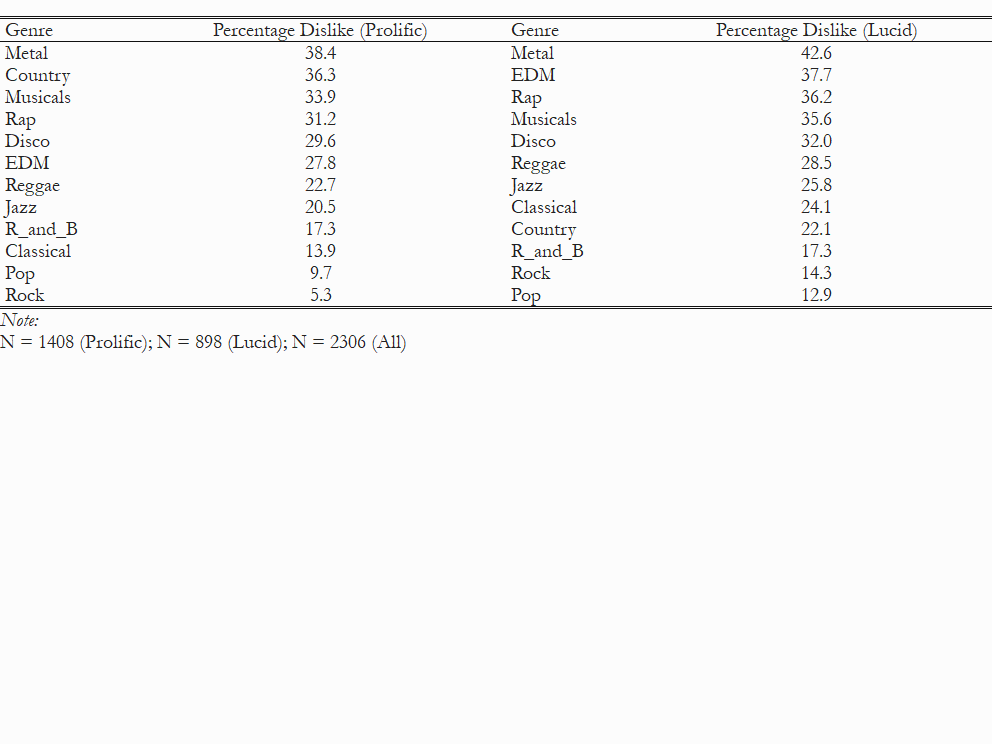
\includegraphics[trim={0 9cm 0 0},clip, width=1.0\textwidth]{Tabs/desc-tab-dislike.png}
    \label{tab:dis-by-genres}
\end{table}

\subsection*{Univariate Distribution of Number of Dislikes}
Table~\ref{tab:dis-dist} shows the univariate distribution of the number of dislikes for both the Prolific and Lucid datasets. As we can see, both datasets agree closely in their estimate of the proportion of categorical tolerants, with the Prolific data returning an estimate of about 19\% of the sample and the Lucid dataset returning an estimate of about 20\%. When we combine both, we get an estimate of 19.6\%, suggesting that about a fifth of the American population today can be classified as categorical tolerants, an increase from L\&S's estimate of about 15\% using data from 2012.\footnote{We should be cautious when making direct comparisons, given that the number of genres included is smaller (twelve versus twenty in L\&S's 2012 survey) in both the Prolific and Lucid samples. Nevertheless, we can at the very least conclude that categorical tolerance remains a pervasive phenomenon among a substantial number of Americans.} 

\begin{table}[ht!]
    \caption{Univariate distribution of dislikes for the Prolific and Lucid samples.}
    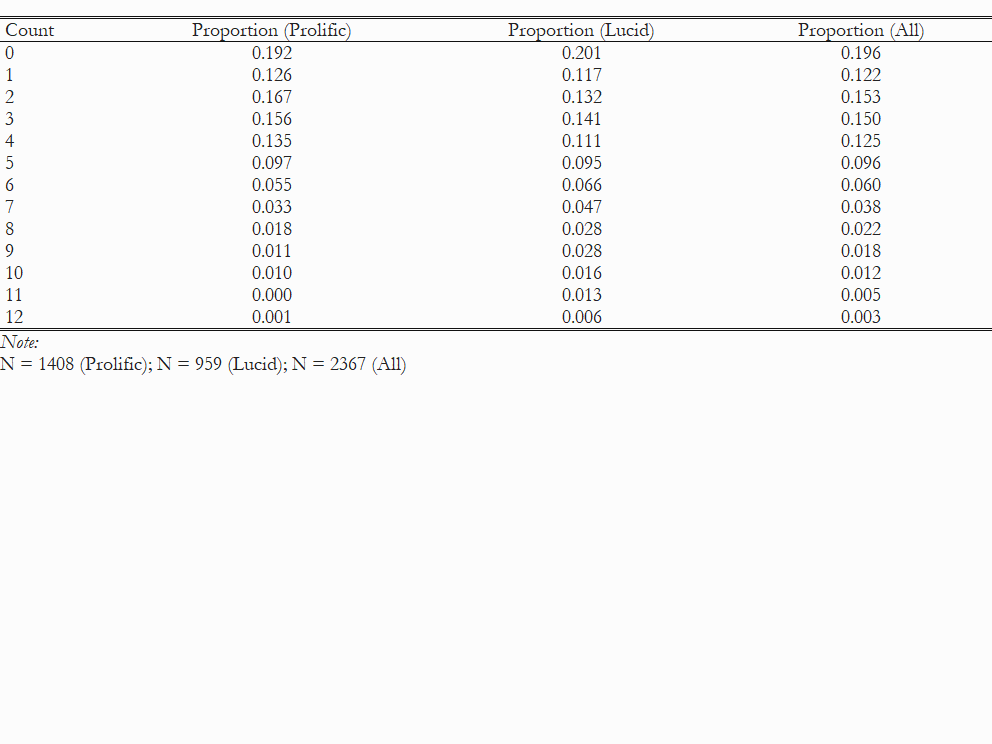
\includegraphics[trim={0 9cm 0 0},clip, width=1.0\textwidth]{Tabs/desc-tab-dislike-dist.png}
    \label{tab:dis-dist}
\end{table}

As shown in Figure~\ref{fig:main}, the distribution of the number of dislikes we get from the joint samples (like the separate sample distributions), exhibits excess zeroes, similar to the one obtained by L\&S using 2012 data. Even considering issues of sample comparability, we can conclude that the taste regime governing patterns of cultural choice among Americans in the second decade of the twenty-first century certainly no longer resembles that captured by the GSS in the early 1990s, with a larger-than-expected---if the number of dislikes followed a simple Poisson process---number of people refusing to express dislikes for any genre. 

\begin{figure}[ht!]
        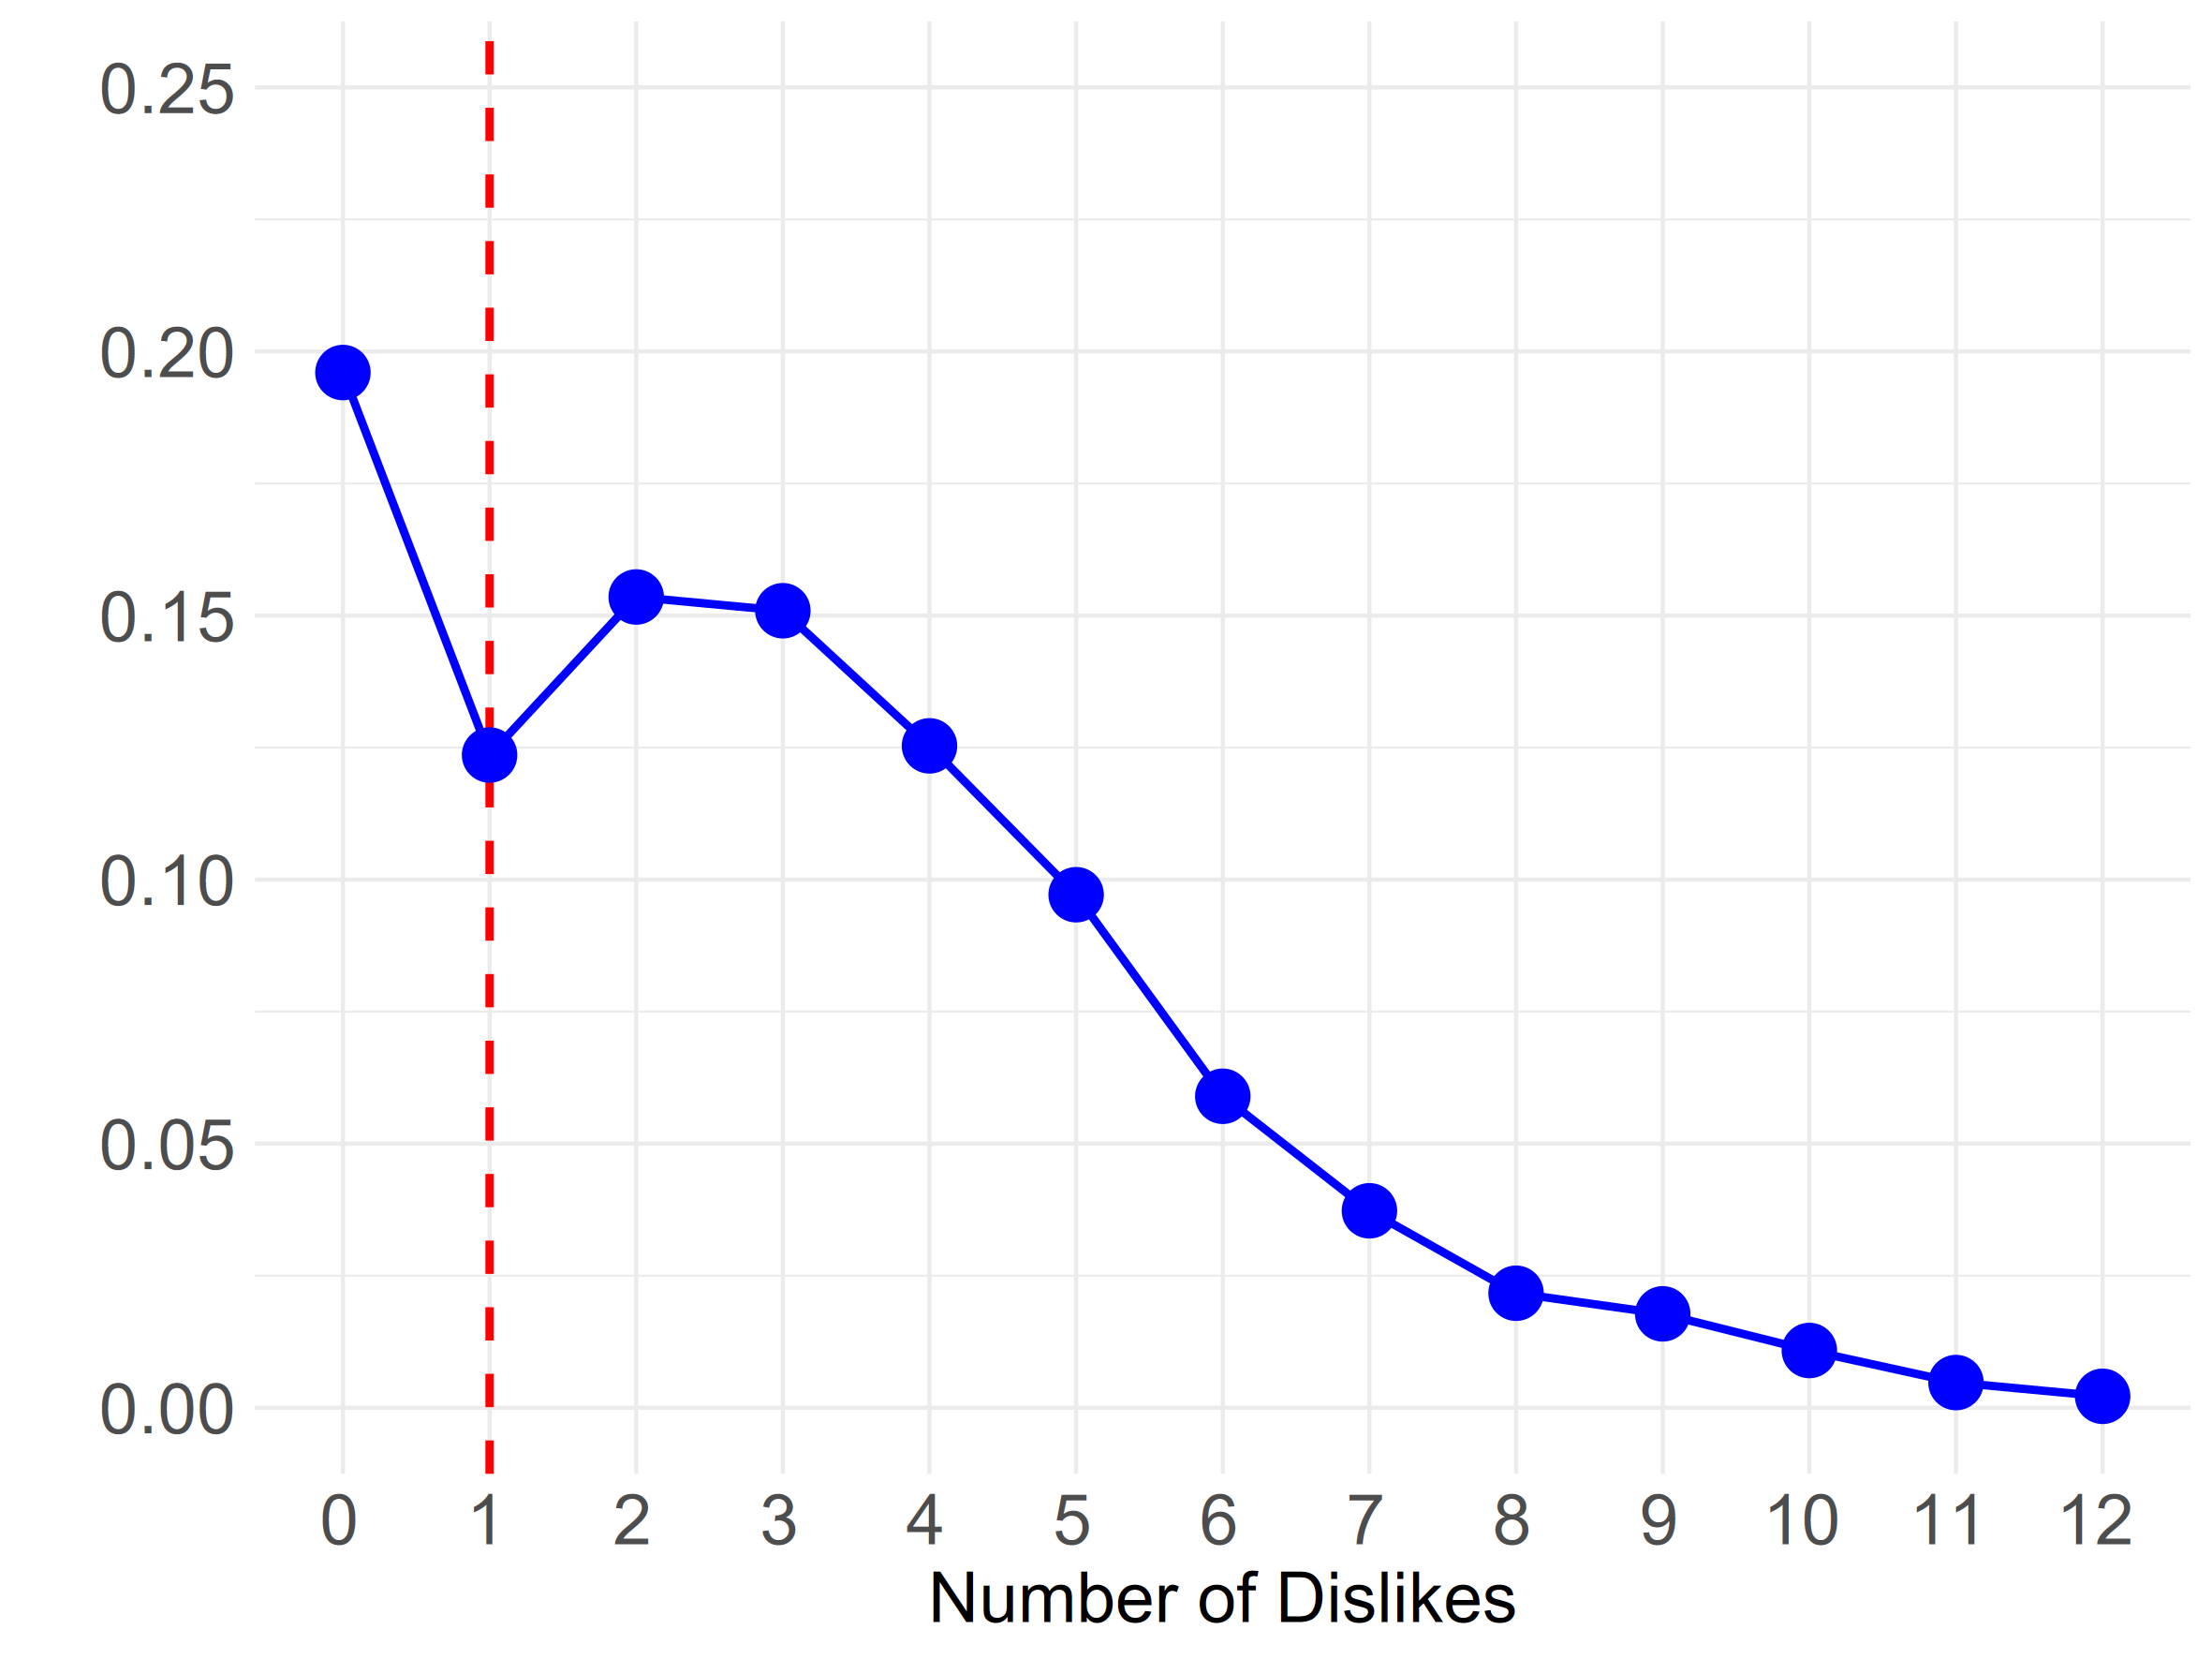
\includegraphics[width=1.0\textwidth]{Plots/uni-dist-cat-tol.png}
    \caption{Univariate plot of number of dislikes, joint Prolific and Lucid samples (N = 2306).}
    \label{fig:main}
\end{figure}

\subsection*{Socio-Demographic Distribution of Categorical Tolerance}
\begin{figure}[ht!]
    \captionsetup[subfigure]{font=footnotesize,labelfont=footnotesize}
    \centering
     \begin{subfigure}[b]{0.3\textwidth}
        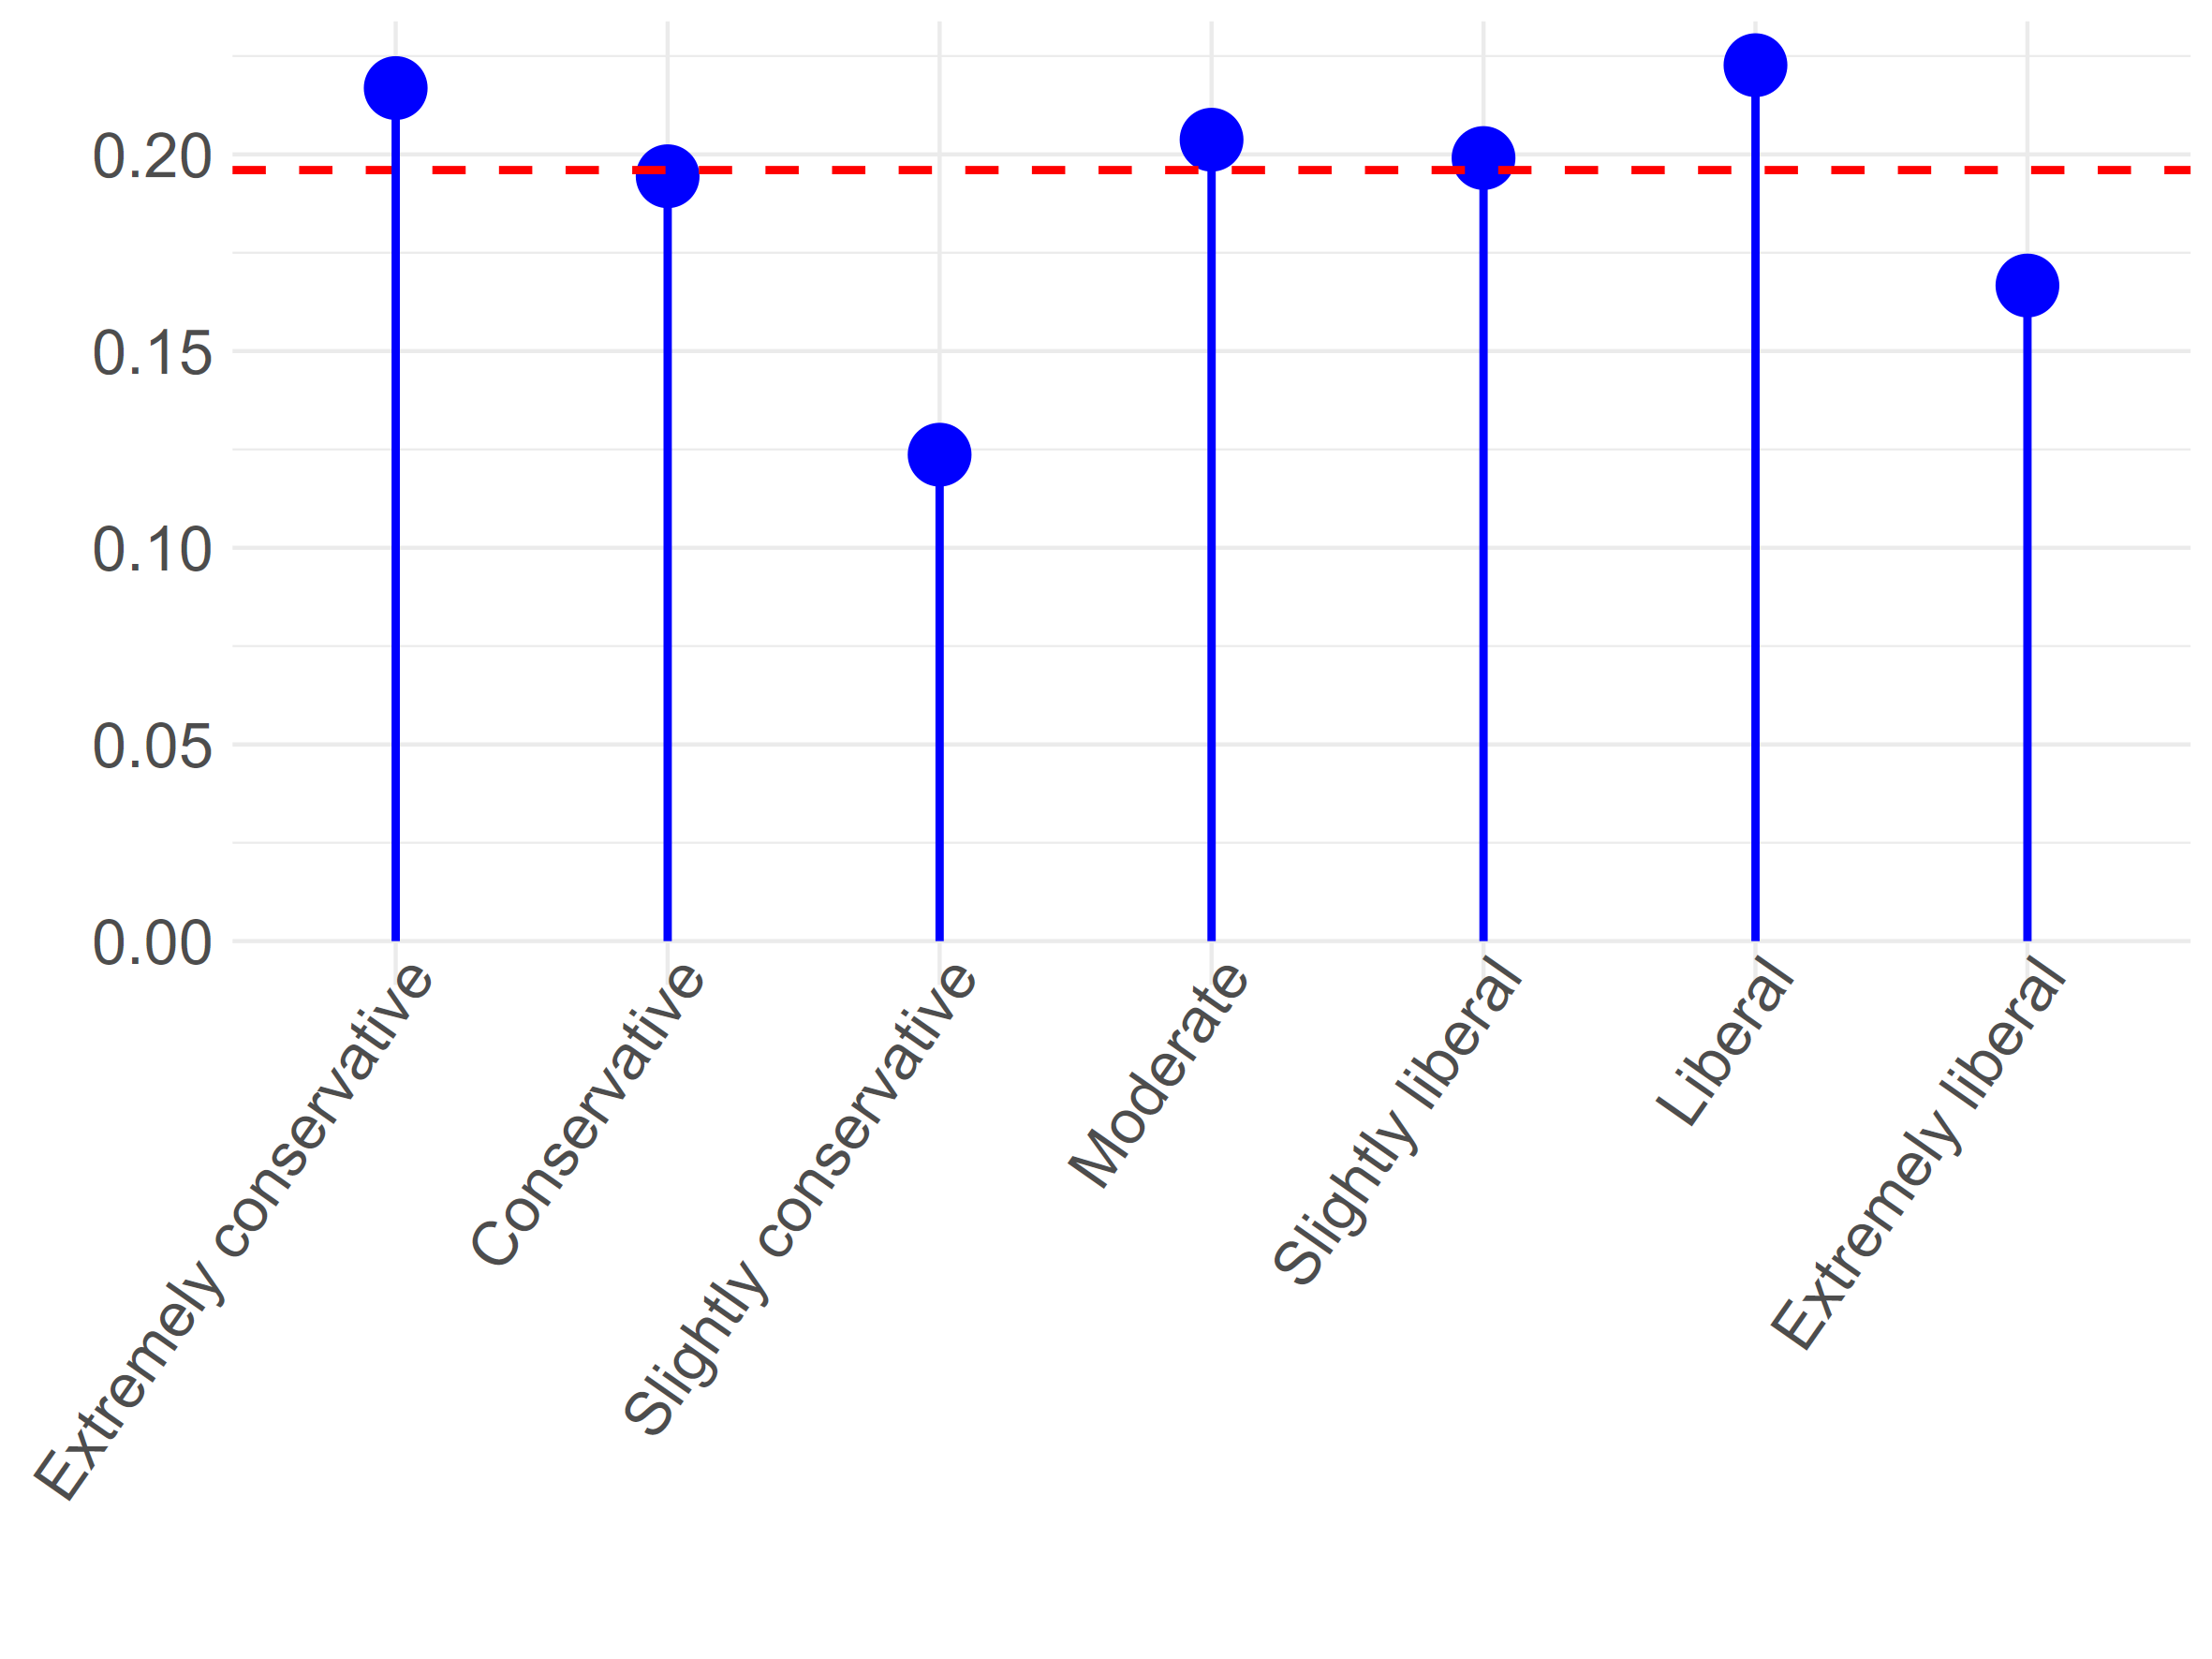
\includegraphics[width=1.0\textwidth]{Plots/uni-dist-cat-tol-pol.png}
            \caption{Political Ideology}
            \label{fig:cat-tol-pol}
    \end{subfigure}
     \begin{subfigure}[b]{0.3\textwidth}
        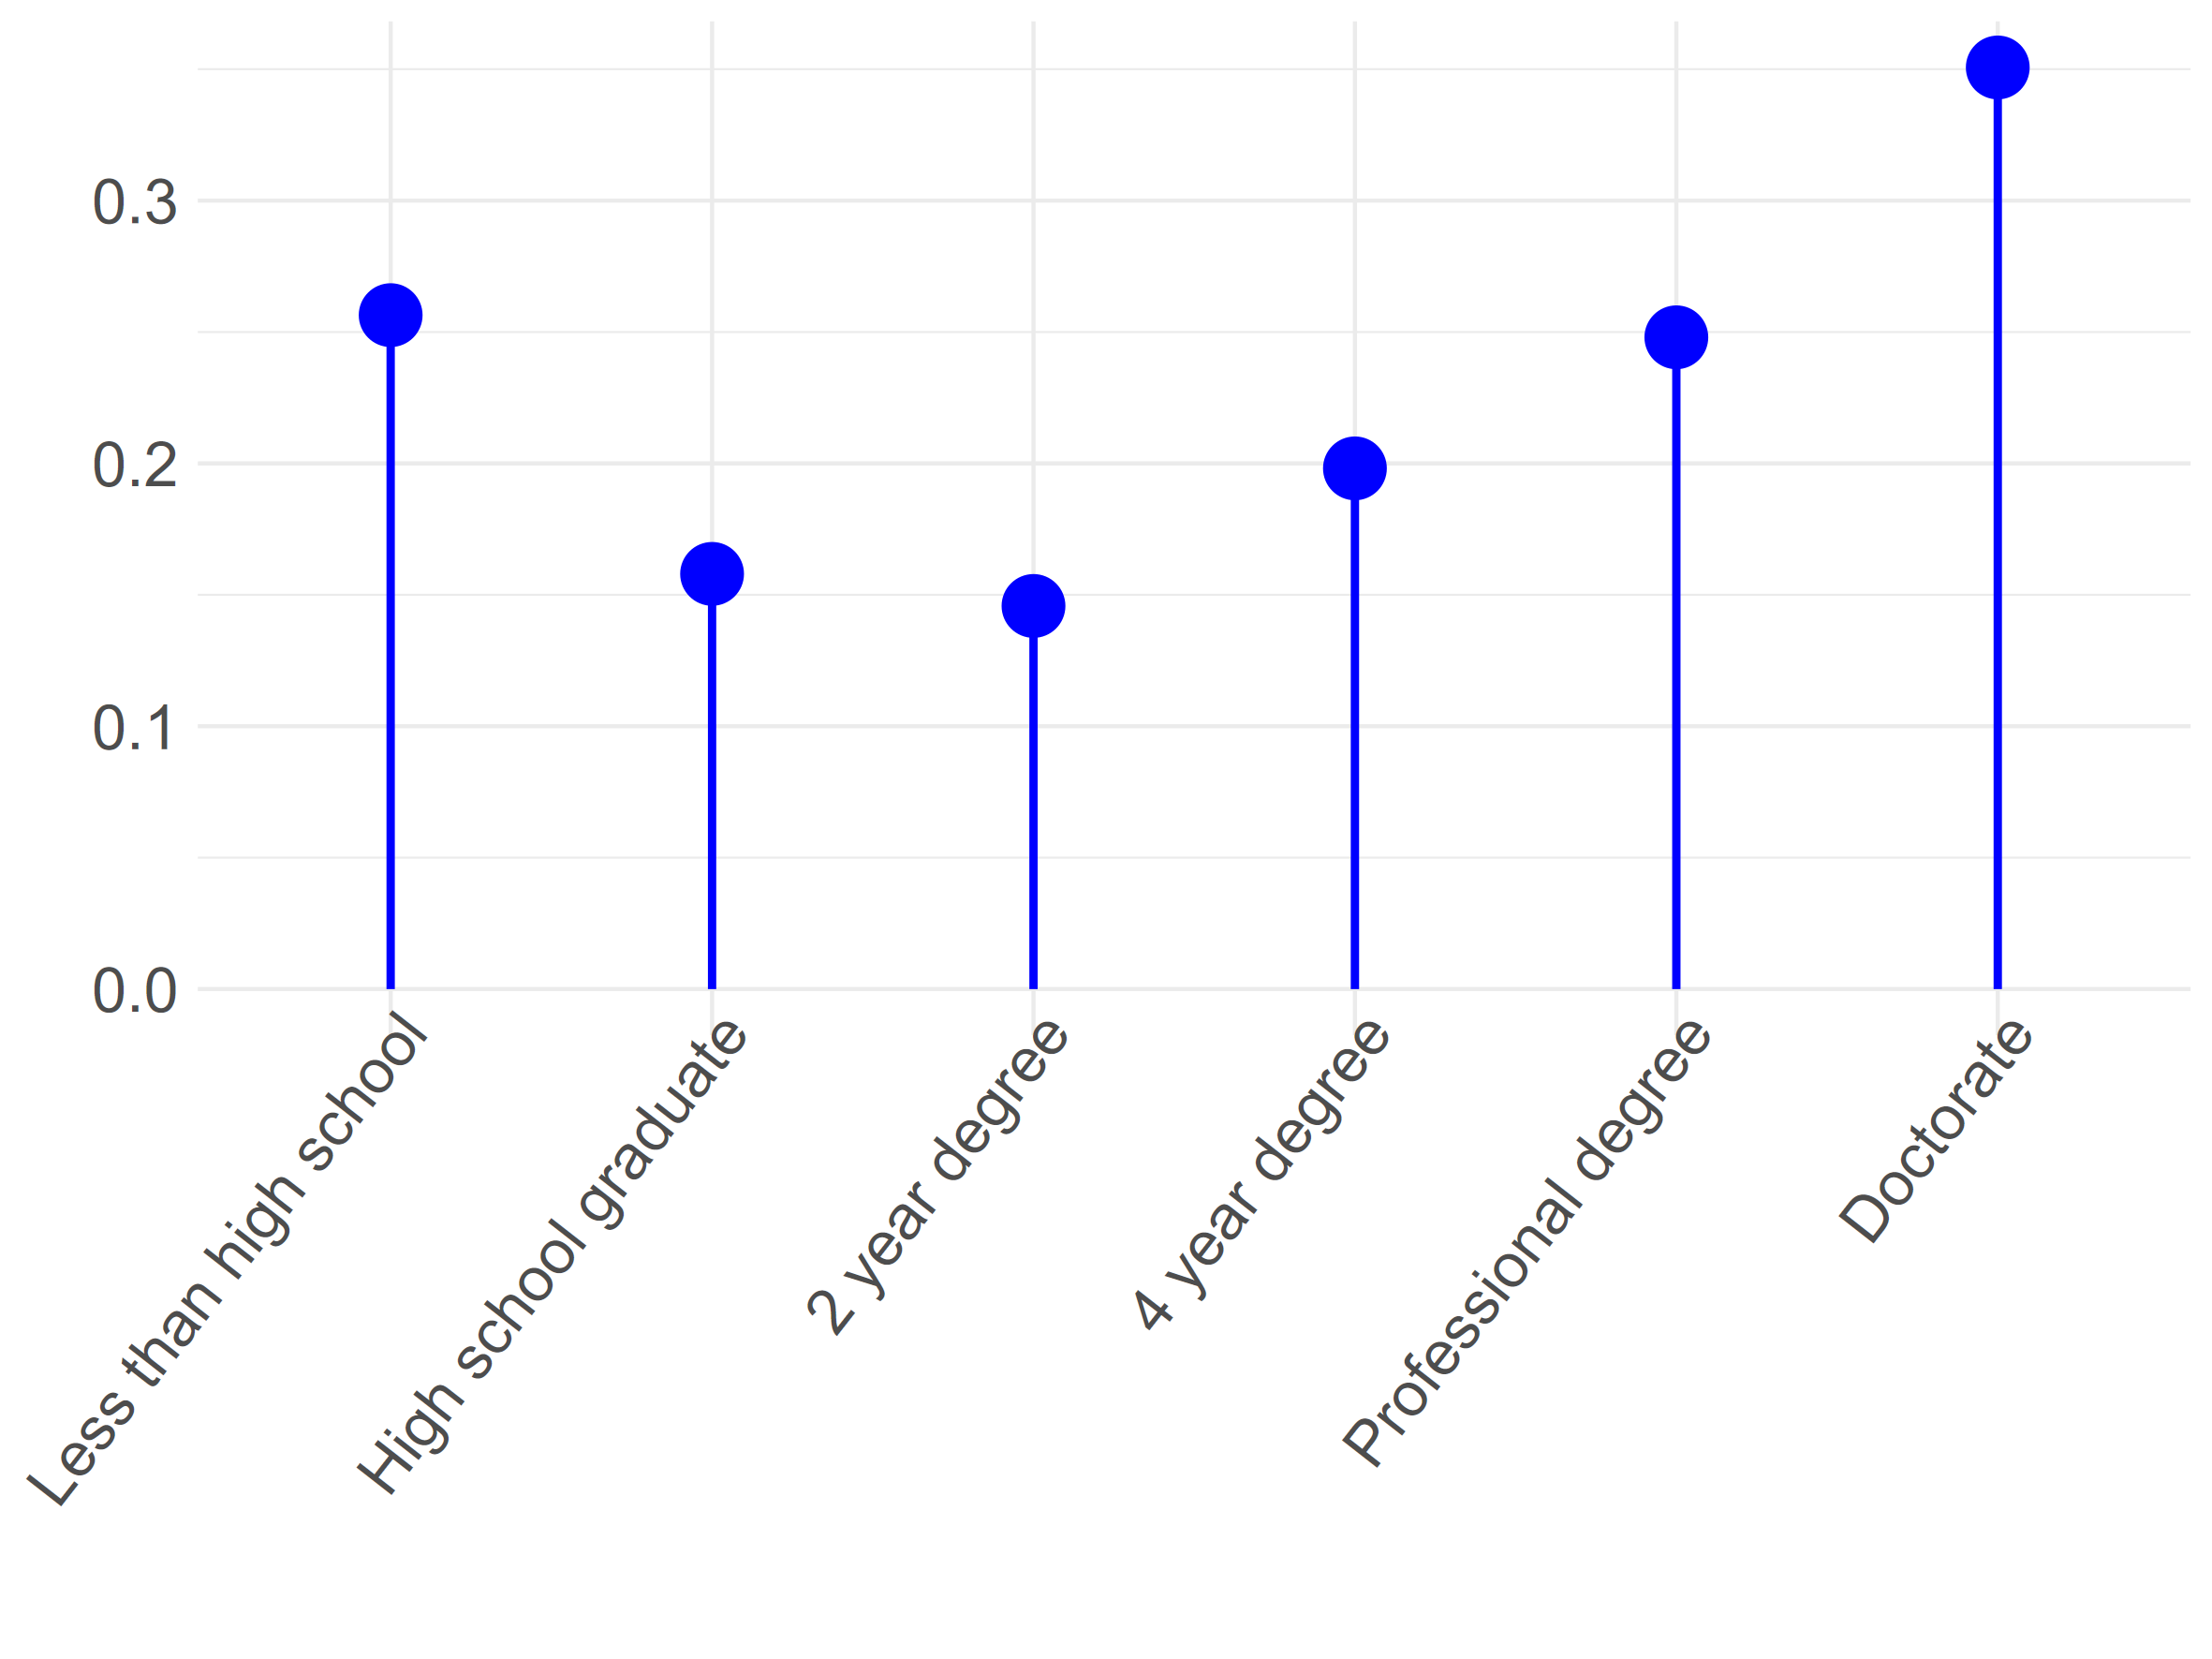
\includegraphics[width=1.0\textwidth]{Plots/uni-dist-cat-tol-edu.png}
            \caption{Education}
            \label{fig:cat-tol-edu}
    \end{subfigure}
     \begin{subfigure}[b]{0.3\textwidth}
        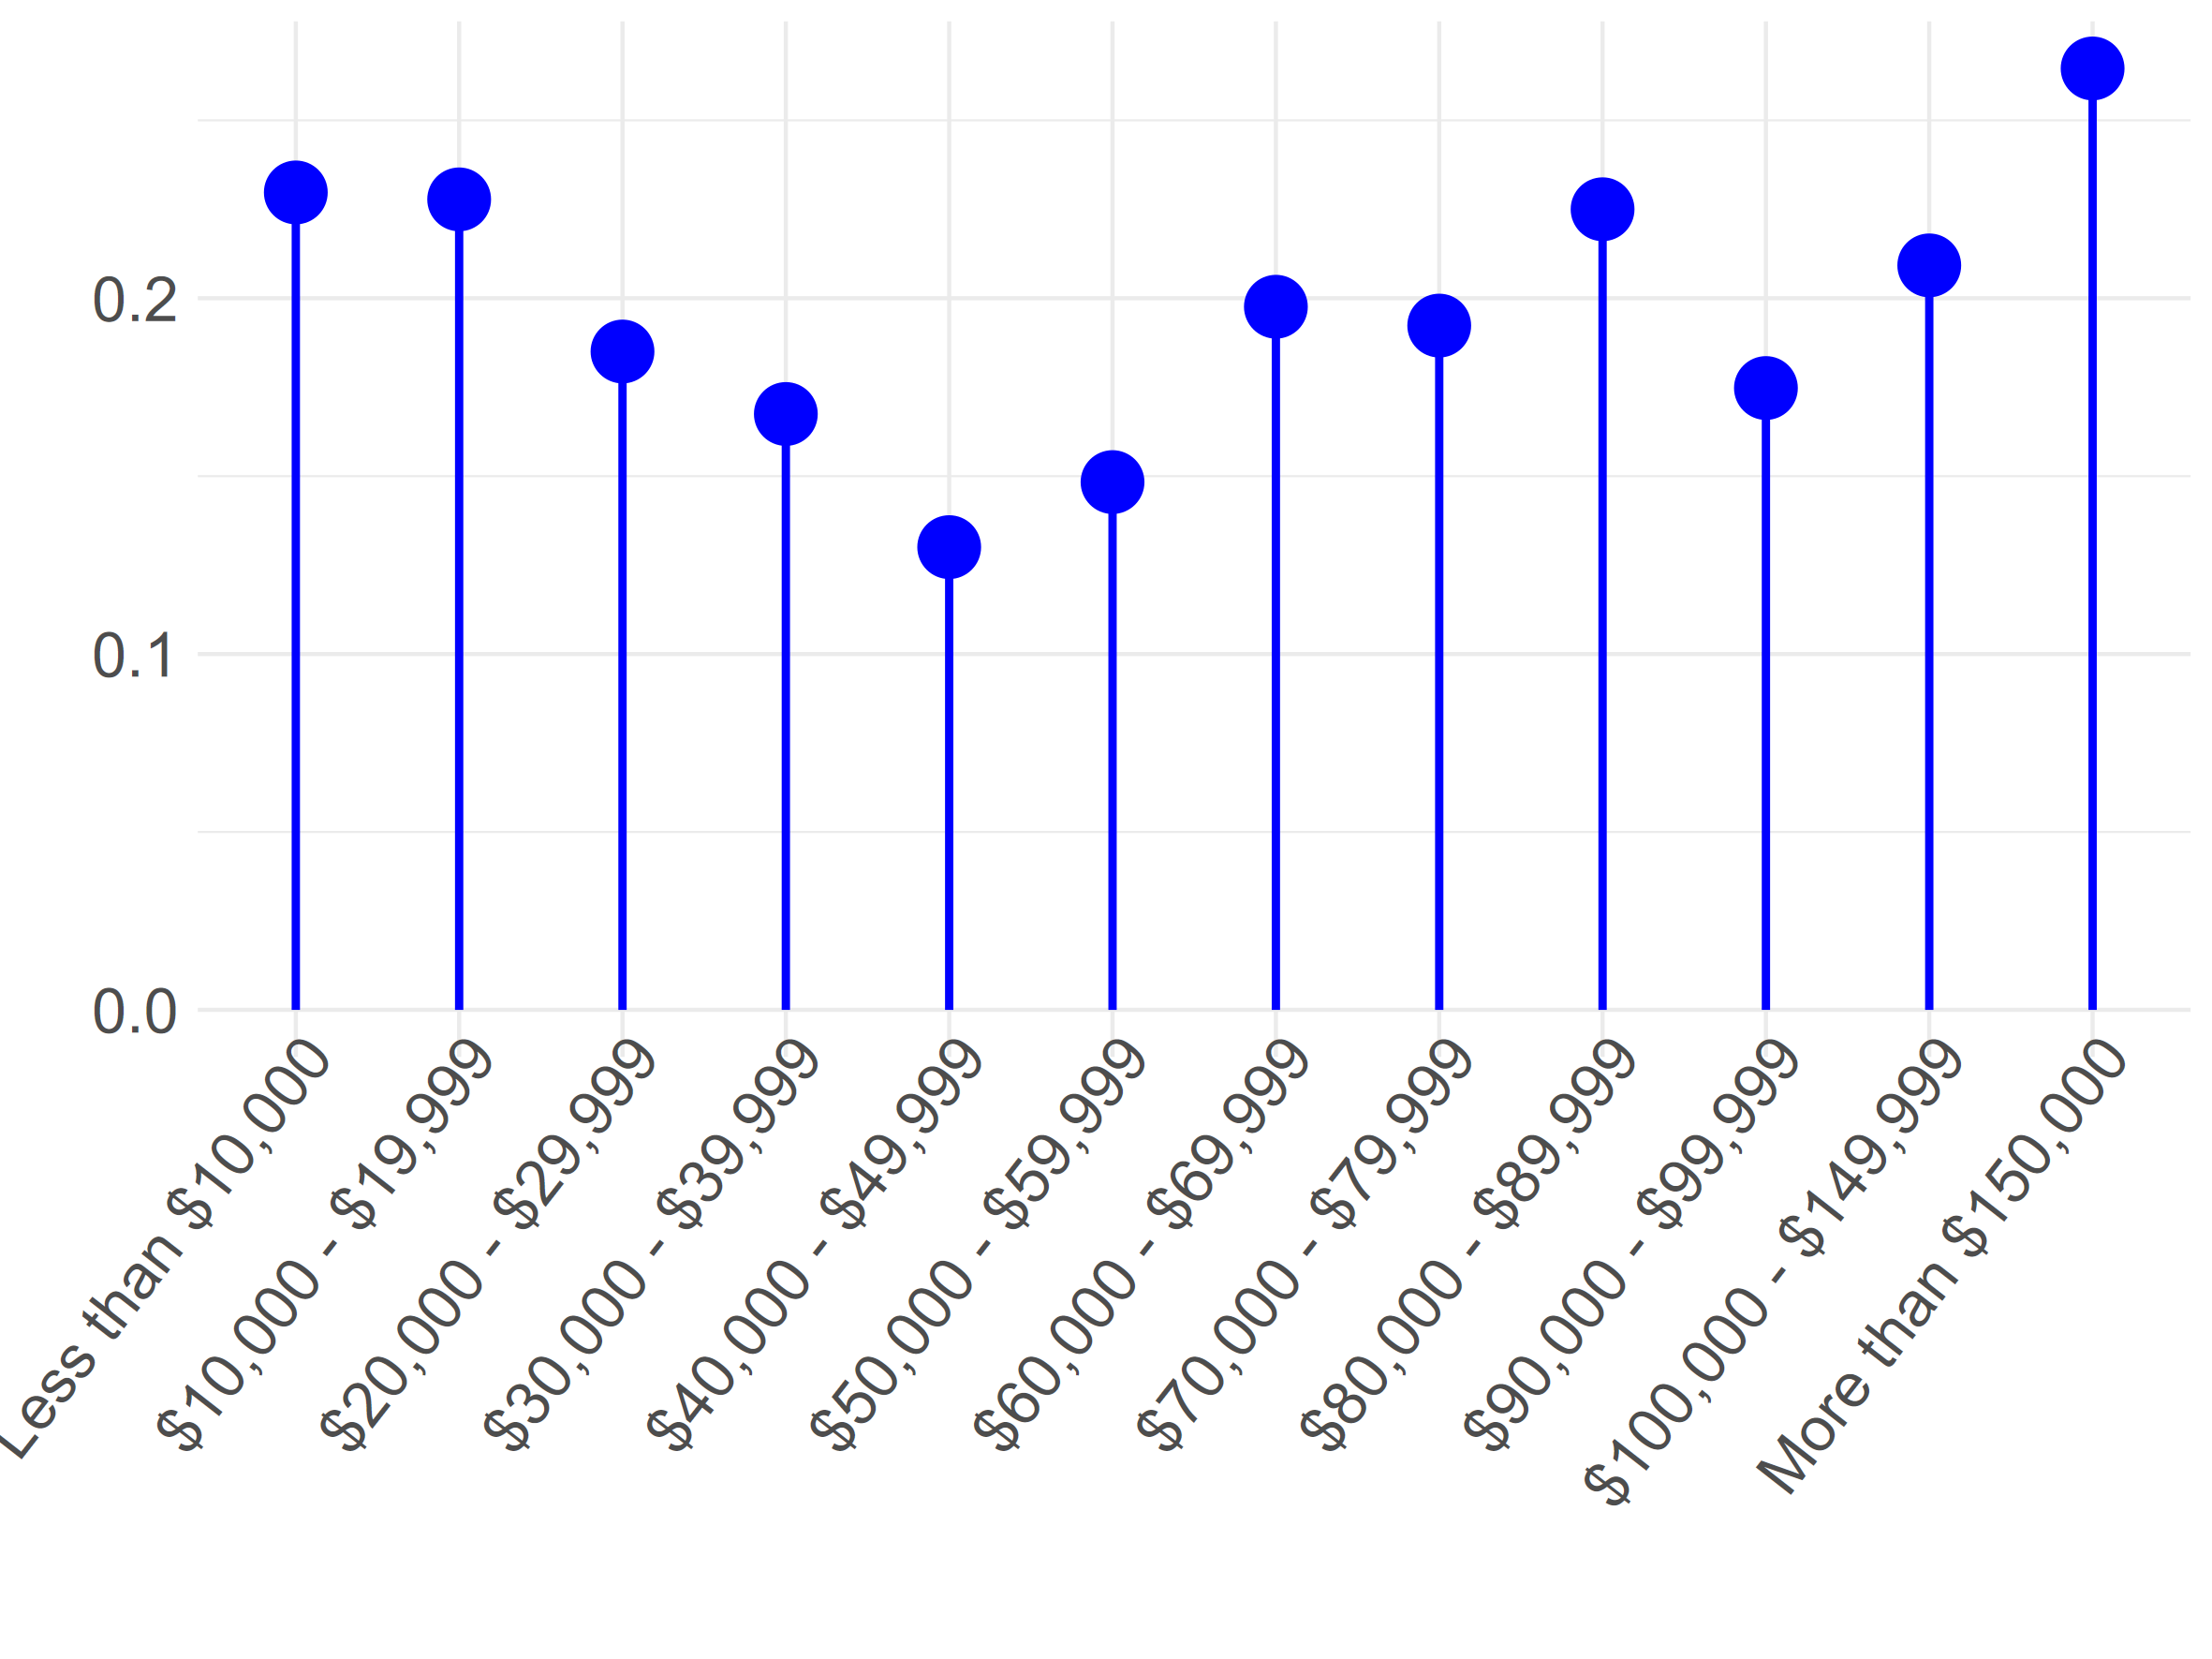
\includegraphics[width=1.0\textwidth]{Plots/uni-dist-cat-tol-inc.png}
            \caption{Income}
            \label{fig:cat-tol-inc}
    \end{subfigure}
     \begin{subfigure}[b]{0.3\textwidth}
        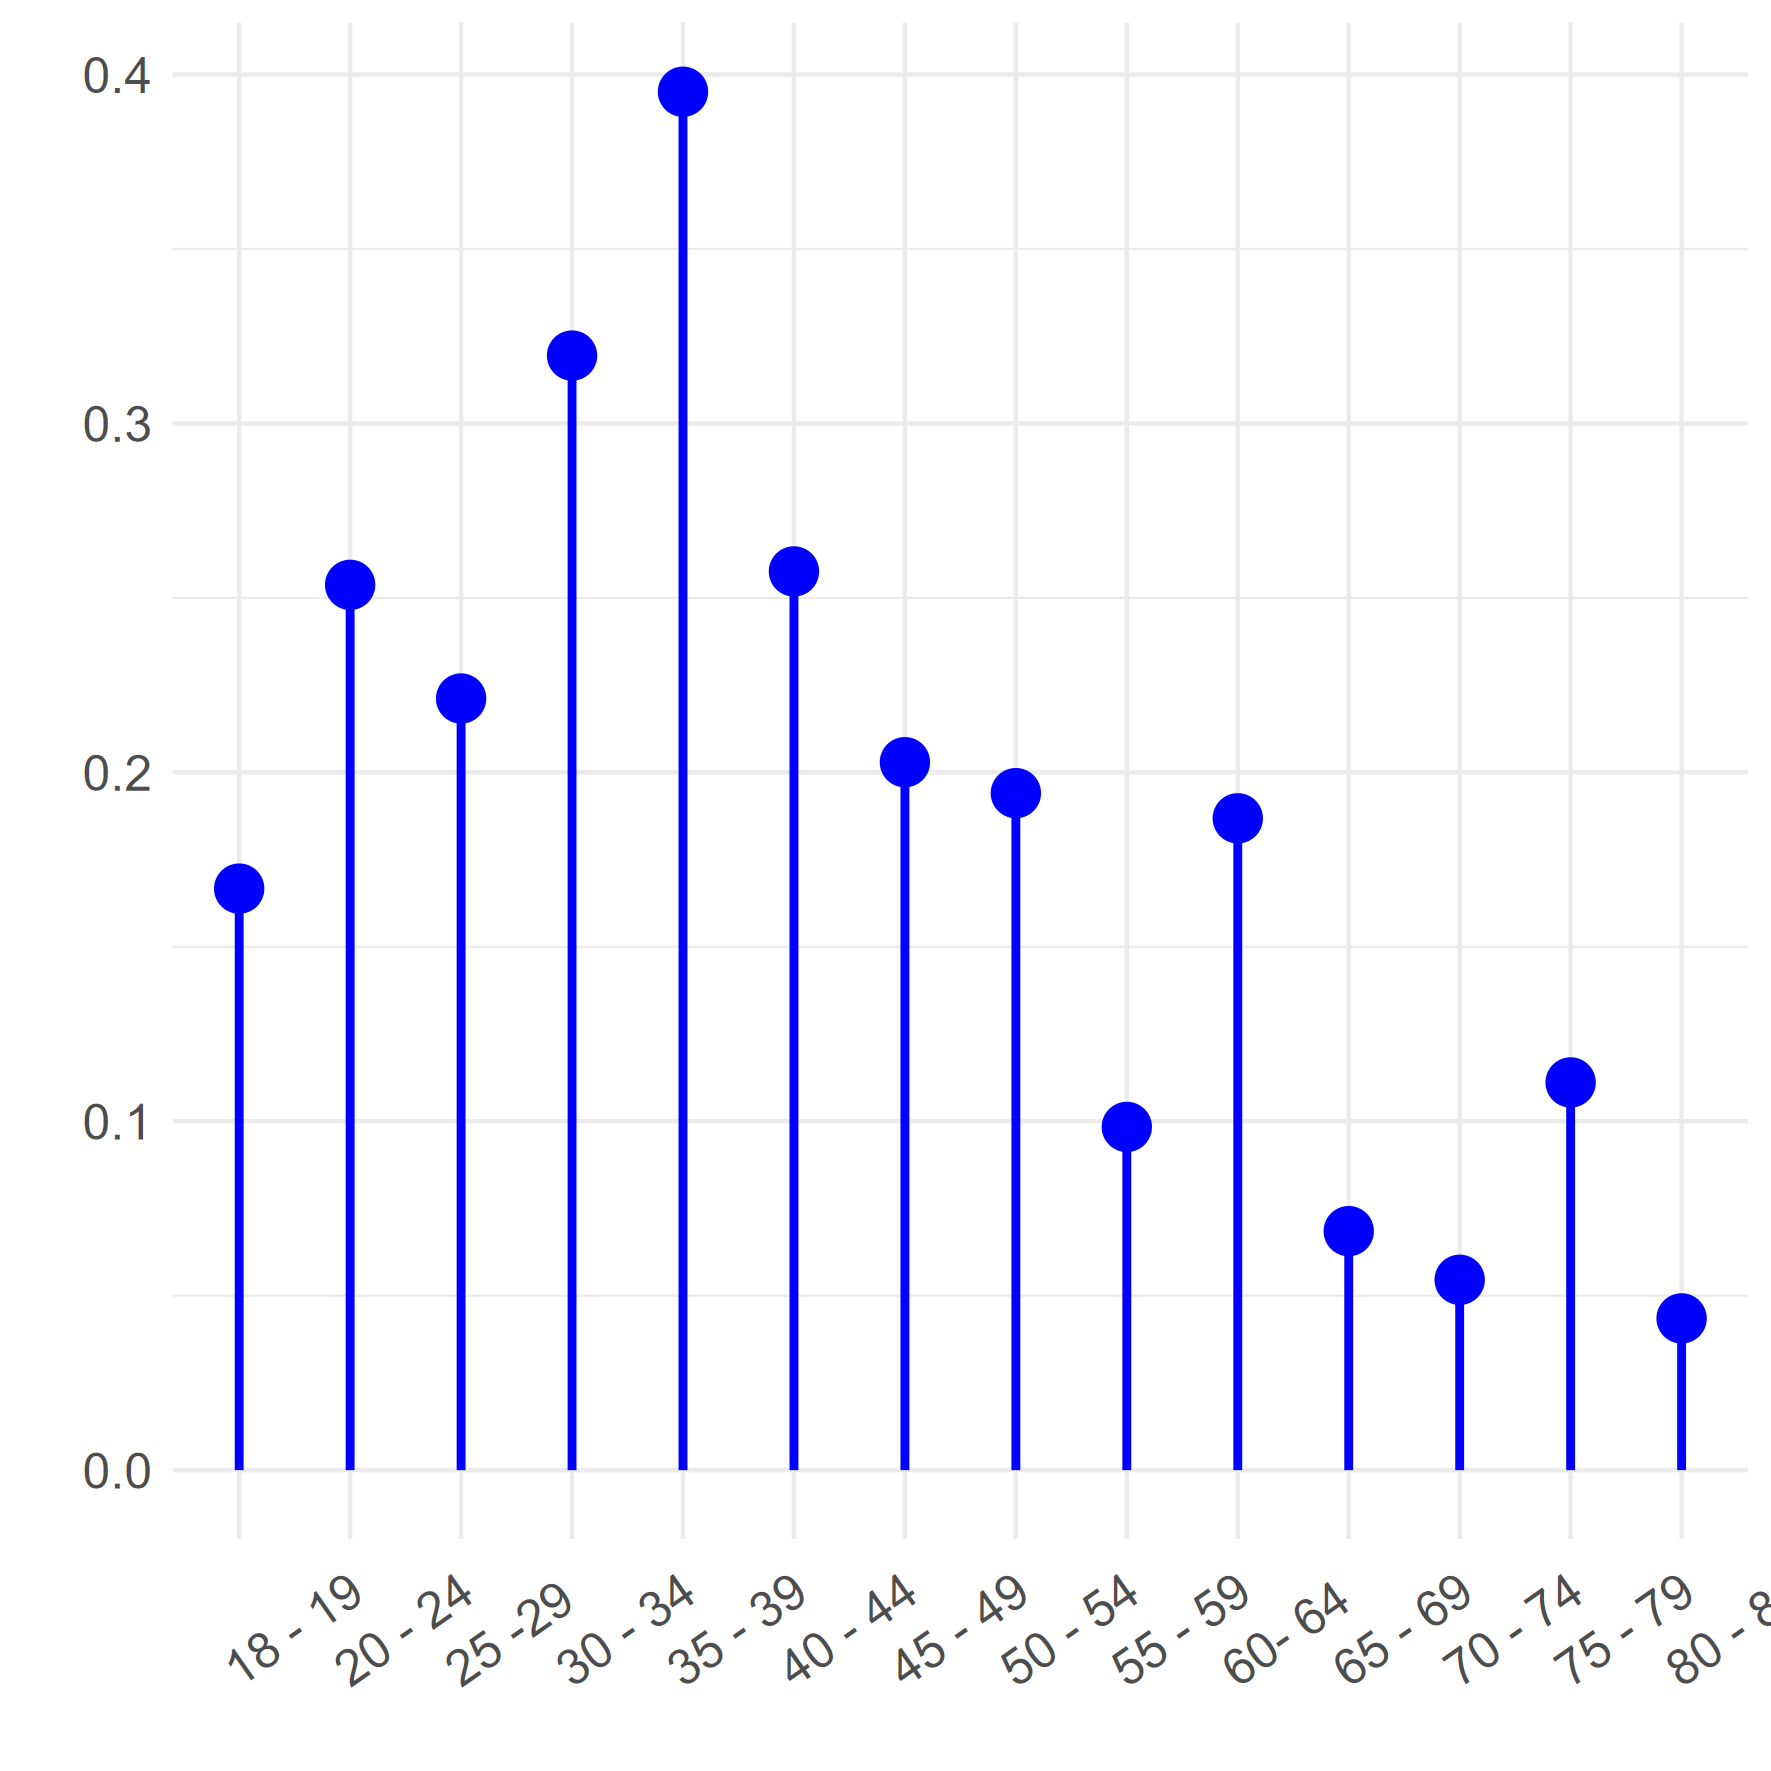
\includegraphics[width=1.0\textwidth]{Plots/uni-dist-cat-tol-age.png}
            \caption{Age}
            \label{fig:cat-tol-age}
    \end{subfigure}
     \begin{subfigure}[b]{0.3\textwidth}
        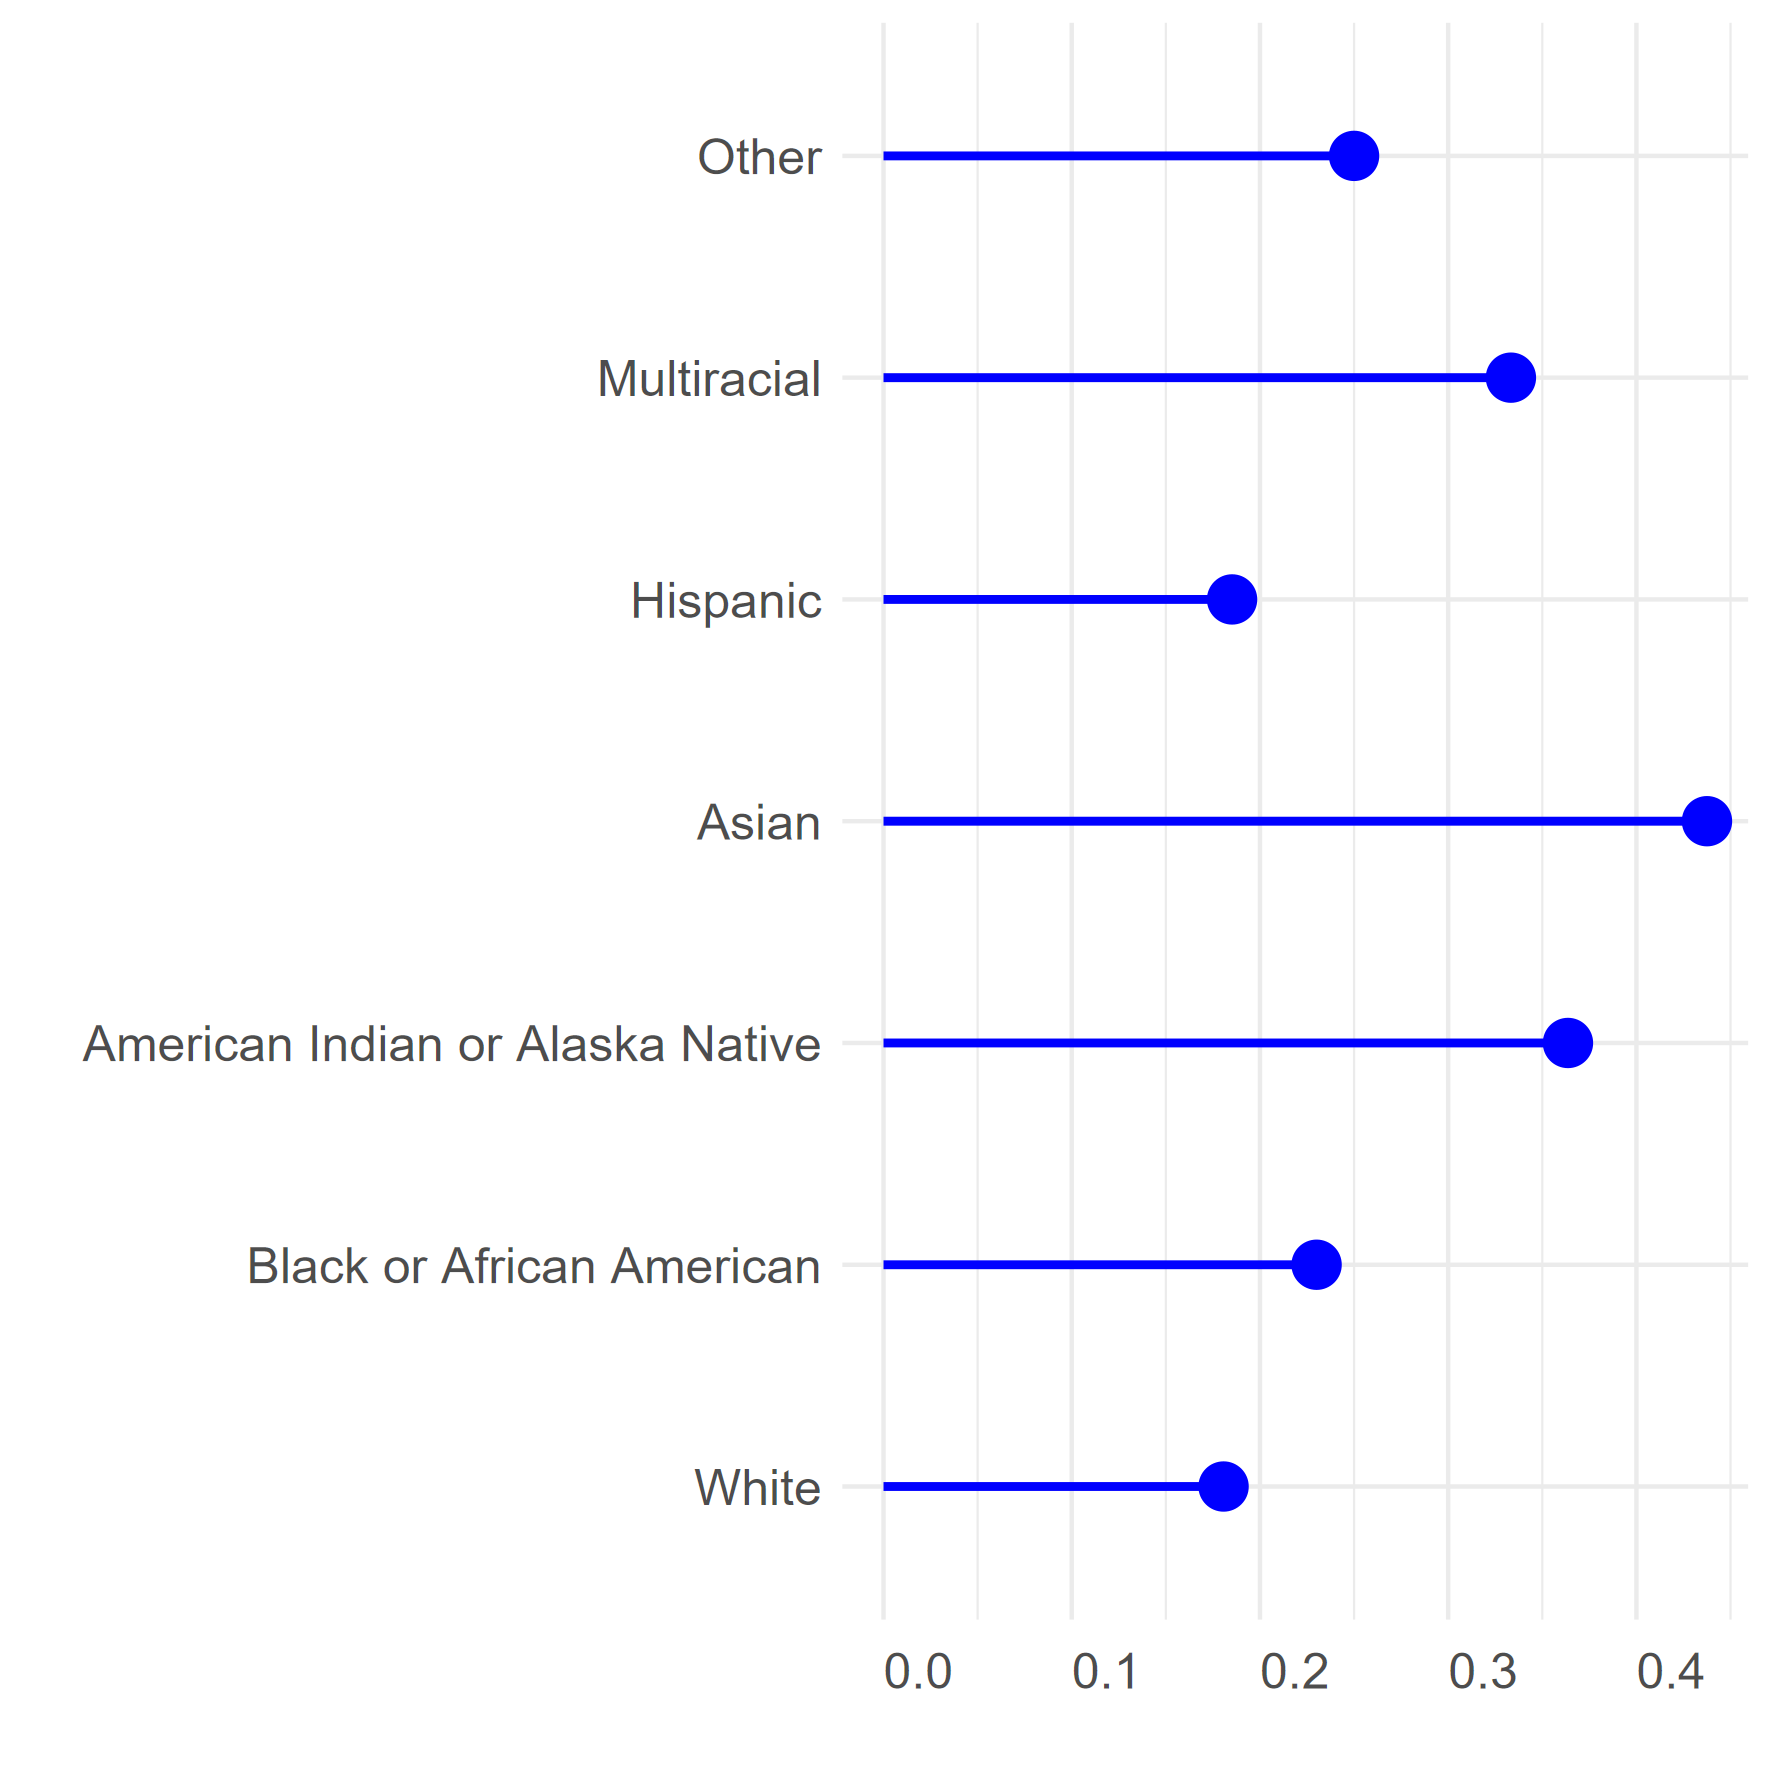
\includegraphics[width=1.0\textwidth]{Plots/uni-dist-cat-tol-rac.png}
            \caption{Ethnoracial Identification}
            \label{fig:cat-tol-rac}
    \end{subfigure}
     \begin{subfigure}[b]{0.3\textwidth}
        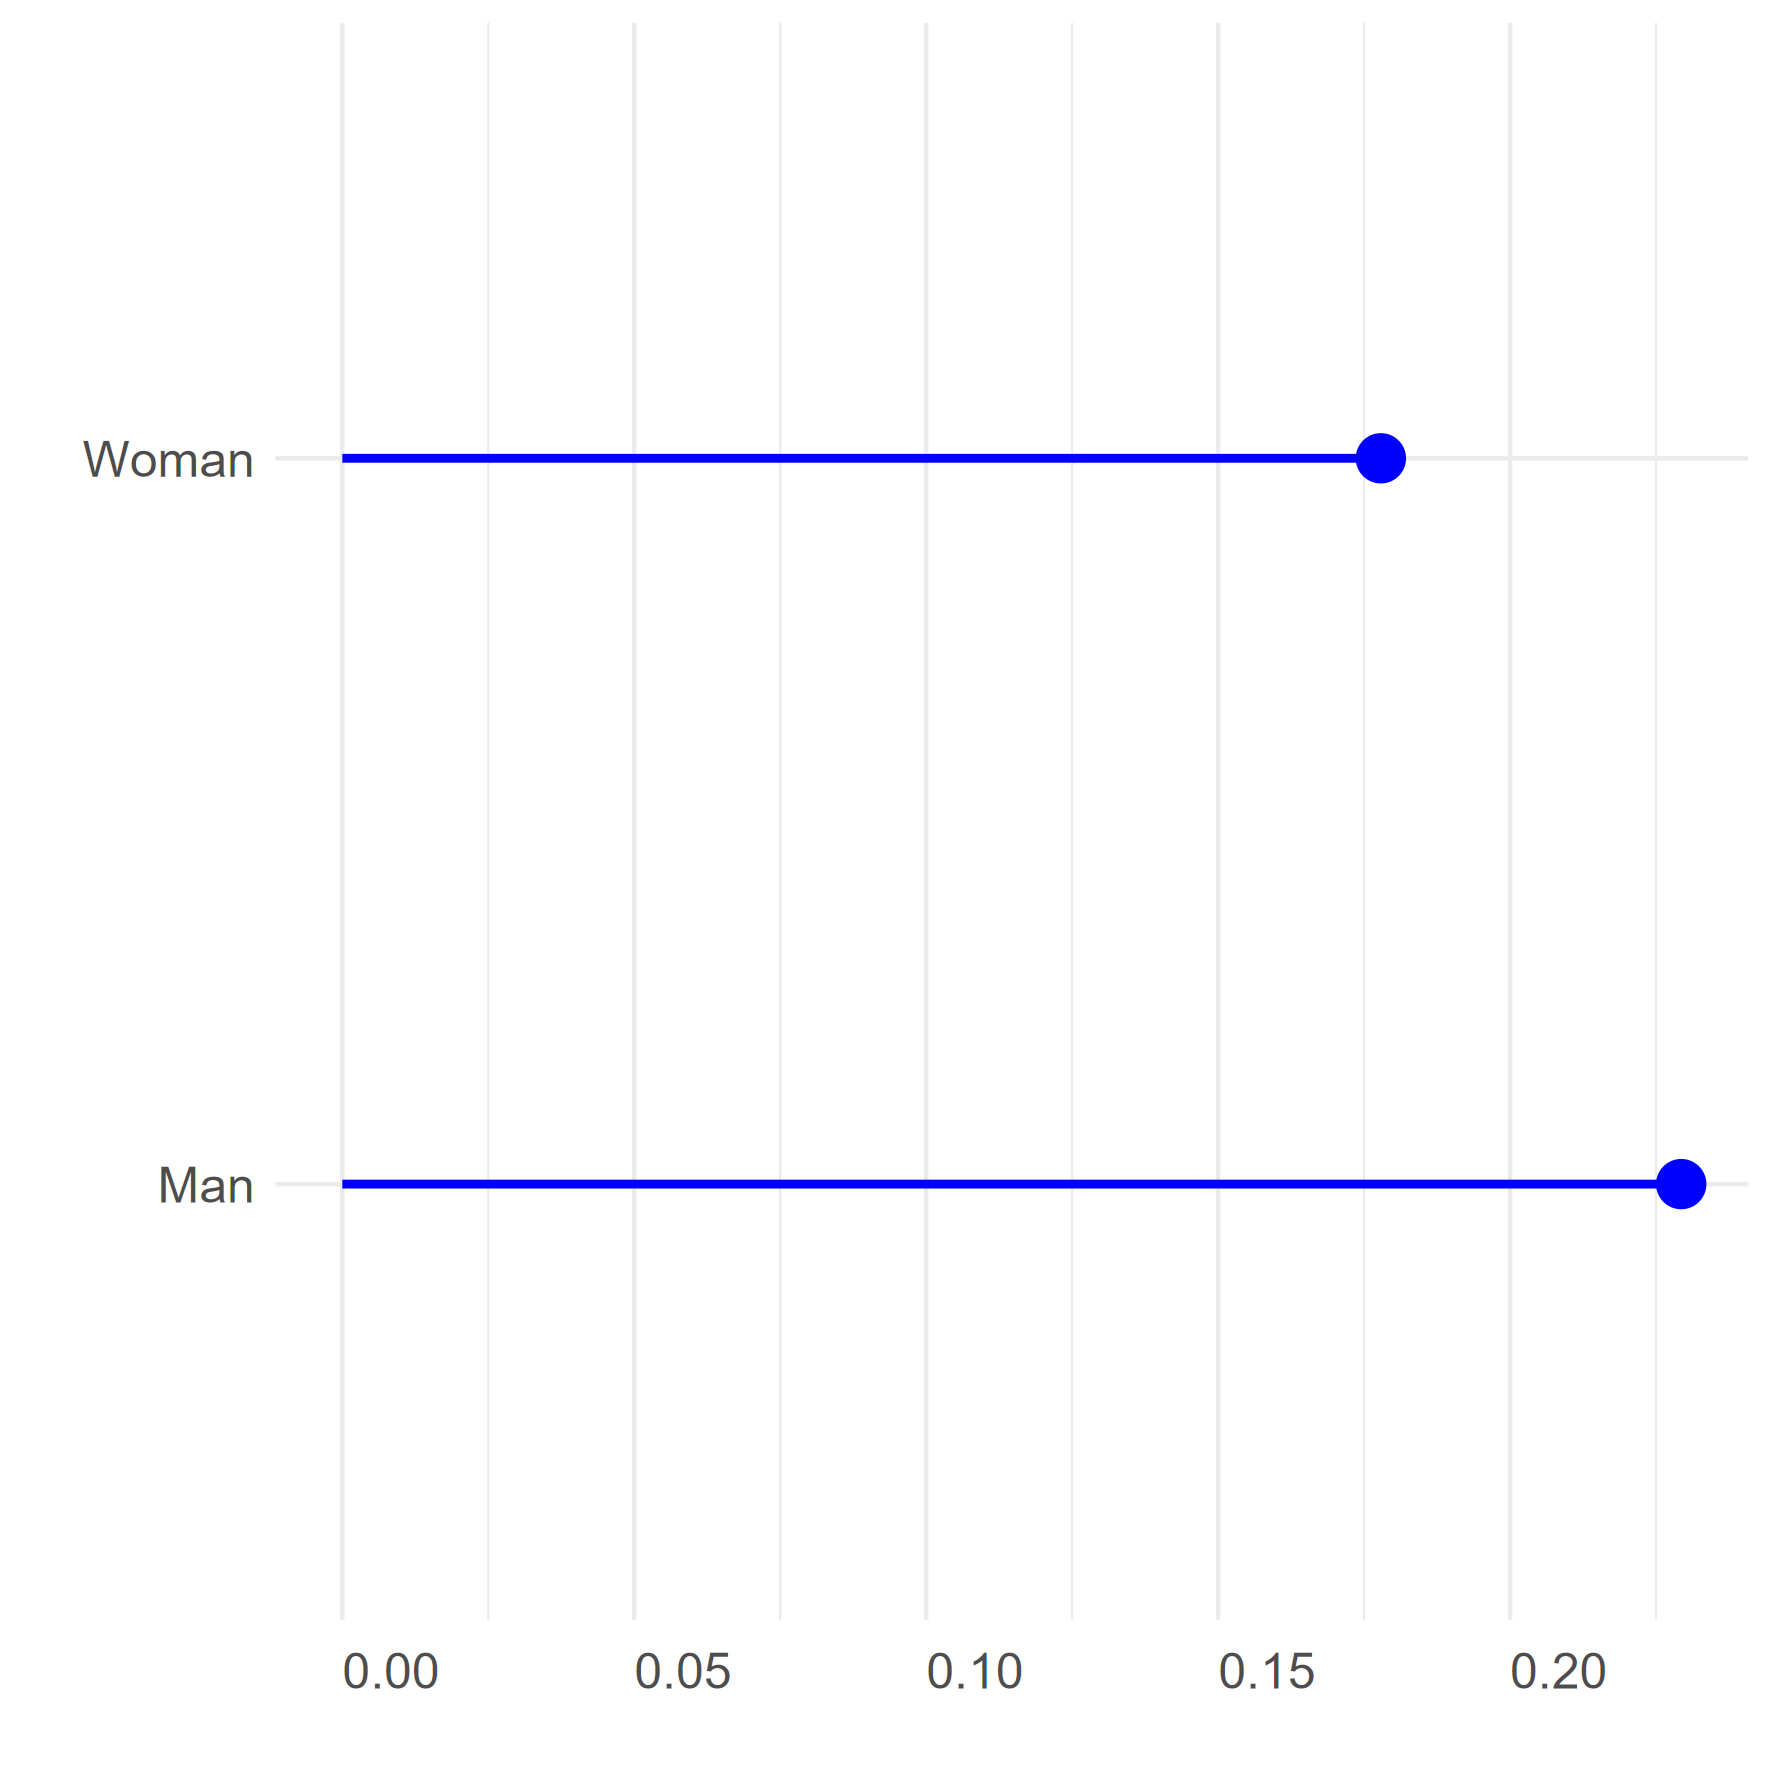
\includegraphics[width=1.0\textwidth]{Plots/uni-dist-cat-tol-gen.png}
            \caption{Gender Identification}
            \label{fig:cat-tol-gen}
    \end{subfigure}
    \caption{Proportion of Categorical Tolerants across different socio-demographic characteristics.}
    \label{fig:cat-tol}
\end{figure}

Figure~\ref{fig:cat-tol} shows how the sample probability of being a categorical tolerant is distributed among various socio-demographic categories. Each panel of Figure~\ref{fig:cat-tol} shows a ``lollipop plot'' with the numerical axis being the proportion of categorical tolerants at each level of the corresponding socio-demographic covariate. The red dashed reference line is the observed sample proportion of categorical tolerants. 

As Figure~\ref{fig:cat-tol-age} shows, age is the most straightforward factor structuring categorical tolerance, replicating the pattern observed by \citet{lizardo2016end-4fb}: Younger people are more likely to be categorical tolerants compared to older people, who are strongly under-represented among categorical tolerants; accordingly, the probability of being a categorical tolerant in these data is maximized among younger adults (individuals in their thirties), suggesting that very young people are induced to use musical genres for purposes of symbolic inclusion to a greater extent than people at this life-stage. Regardless, it is clear that if cohort replacement dynamics drive the rise of categorical tolerance, then we should expect it to remain a fixture of the cultural taste landscape in the U.S. as older, less categorically tolerant cohorts exit the population. 

The other obvious factor structuring categorical tolerance in the United States is race. Mirroring L\&S's earlier findings, Figure~\ref{fig:cat-tol-rac} shows that categorical tolerance continues to be primarily a non-white phenomenon, with whites (and to a similar extent respondents who identify as Hispanic) under-represented among categorical tolerants, and Black, Asian, and Native American respondents over-represented. Also similar to L\&S's findings, the traditional Bourdieusian structuring factors (e.g., education and income) do not have a straightforward link to categorical tolerance, with both showing non-linear patterns (categorical tolerants over-represented among both high and low education and high and low-income respondents). Interestingly, we also observe a strong gender effect — unlike L\&S's earlier findings — which suggests a relatively large gender gap in this taste pattern, with men overrepresented and women underrepresented among the ranks of categorical tolerants. Finally, and also consequentially, categorical tolerance---in contrast to symbolic exclusion as we will see in a bit---is not polarized along political-ideological lines, with no clear pattern shown according to conservative/liberal placement. 

\subsection*{Socio-Demographic Distribution of Symbolic Exclusion}
The obverse phenomenon of categorical tolerance is \emph{symbolic exclusion} \citep{bryson1996anything-311}, that is, the probability of expressing at least one dislike, among those in the population who are at risk of doing so. Figure~\ref{fig:grd-int} shows the distribution of symbolic exclusion propensities in the joint Prolific and Lucid sample using a similar plotting strategy as Figure~\ref{fig:cat-tol}, but this time with the average number of dislikes expressed by members of each socio-demographic category in the numerical axis. The dashed red reference line, like before, represents the average number of dislikes among individuals in the joint sample. 

\begin{figure}[ht!]
    \captionsetup[subfigure]{font=footnotesize,labelfont=footnotesize}
    \centering
     \begin{subfigure}[b]{0.3\textwidth}
        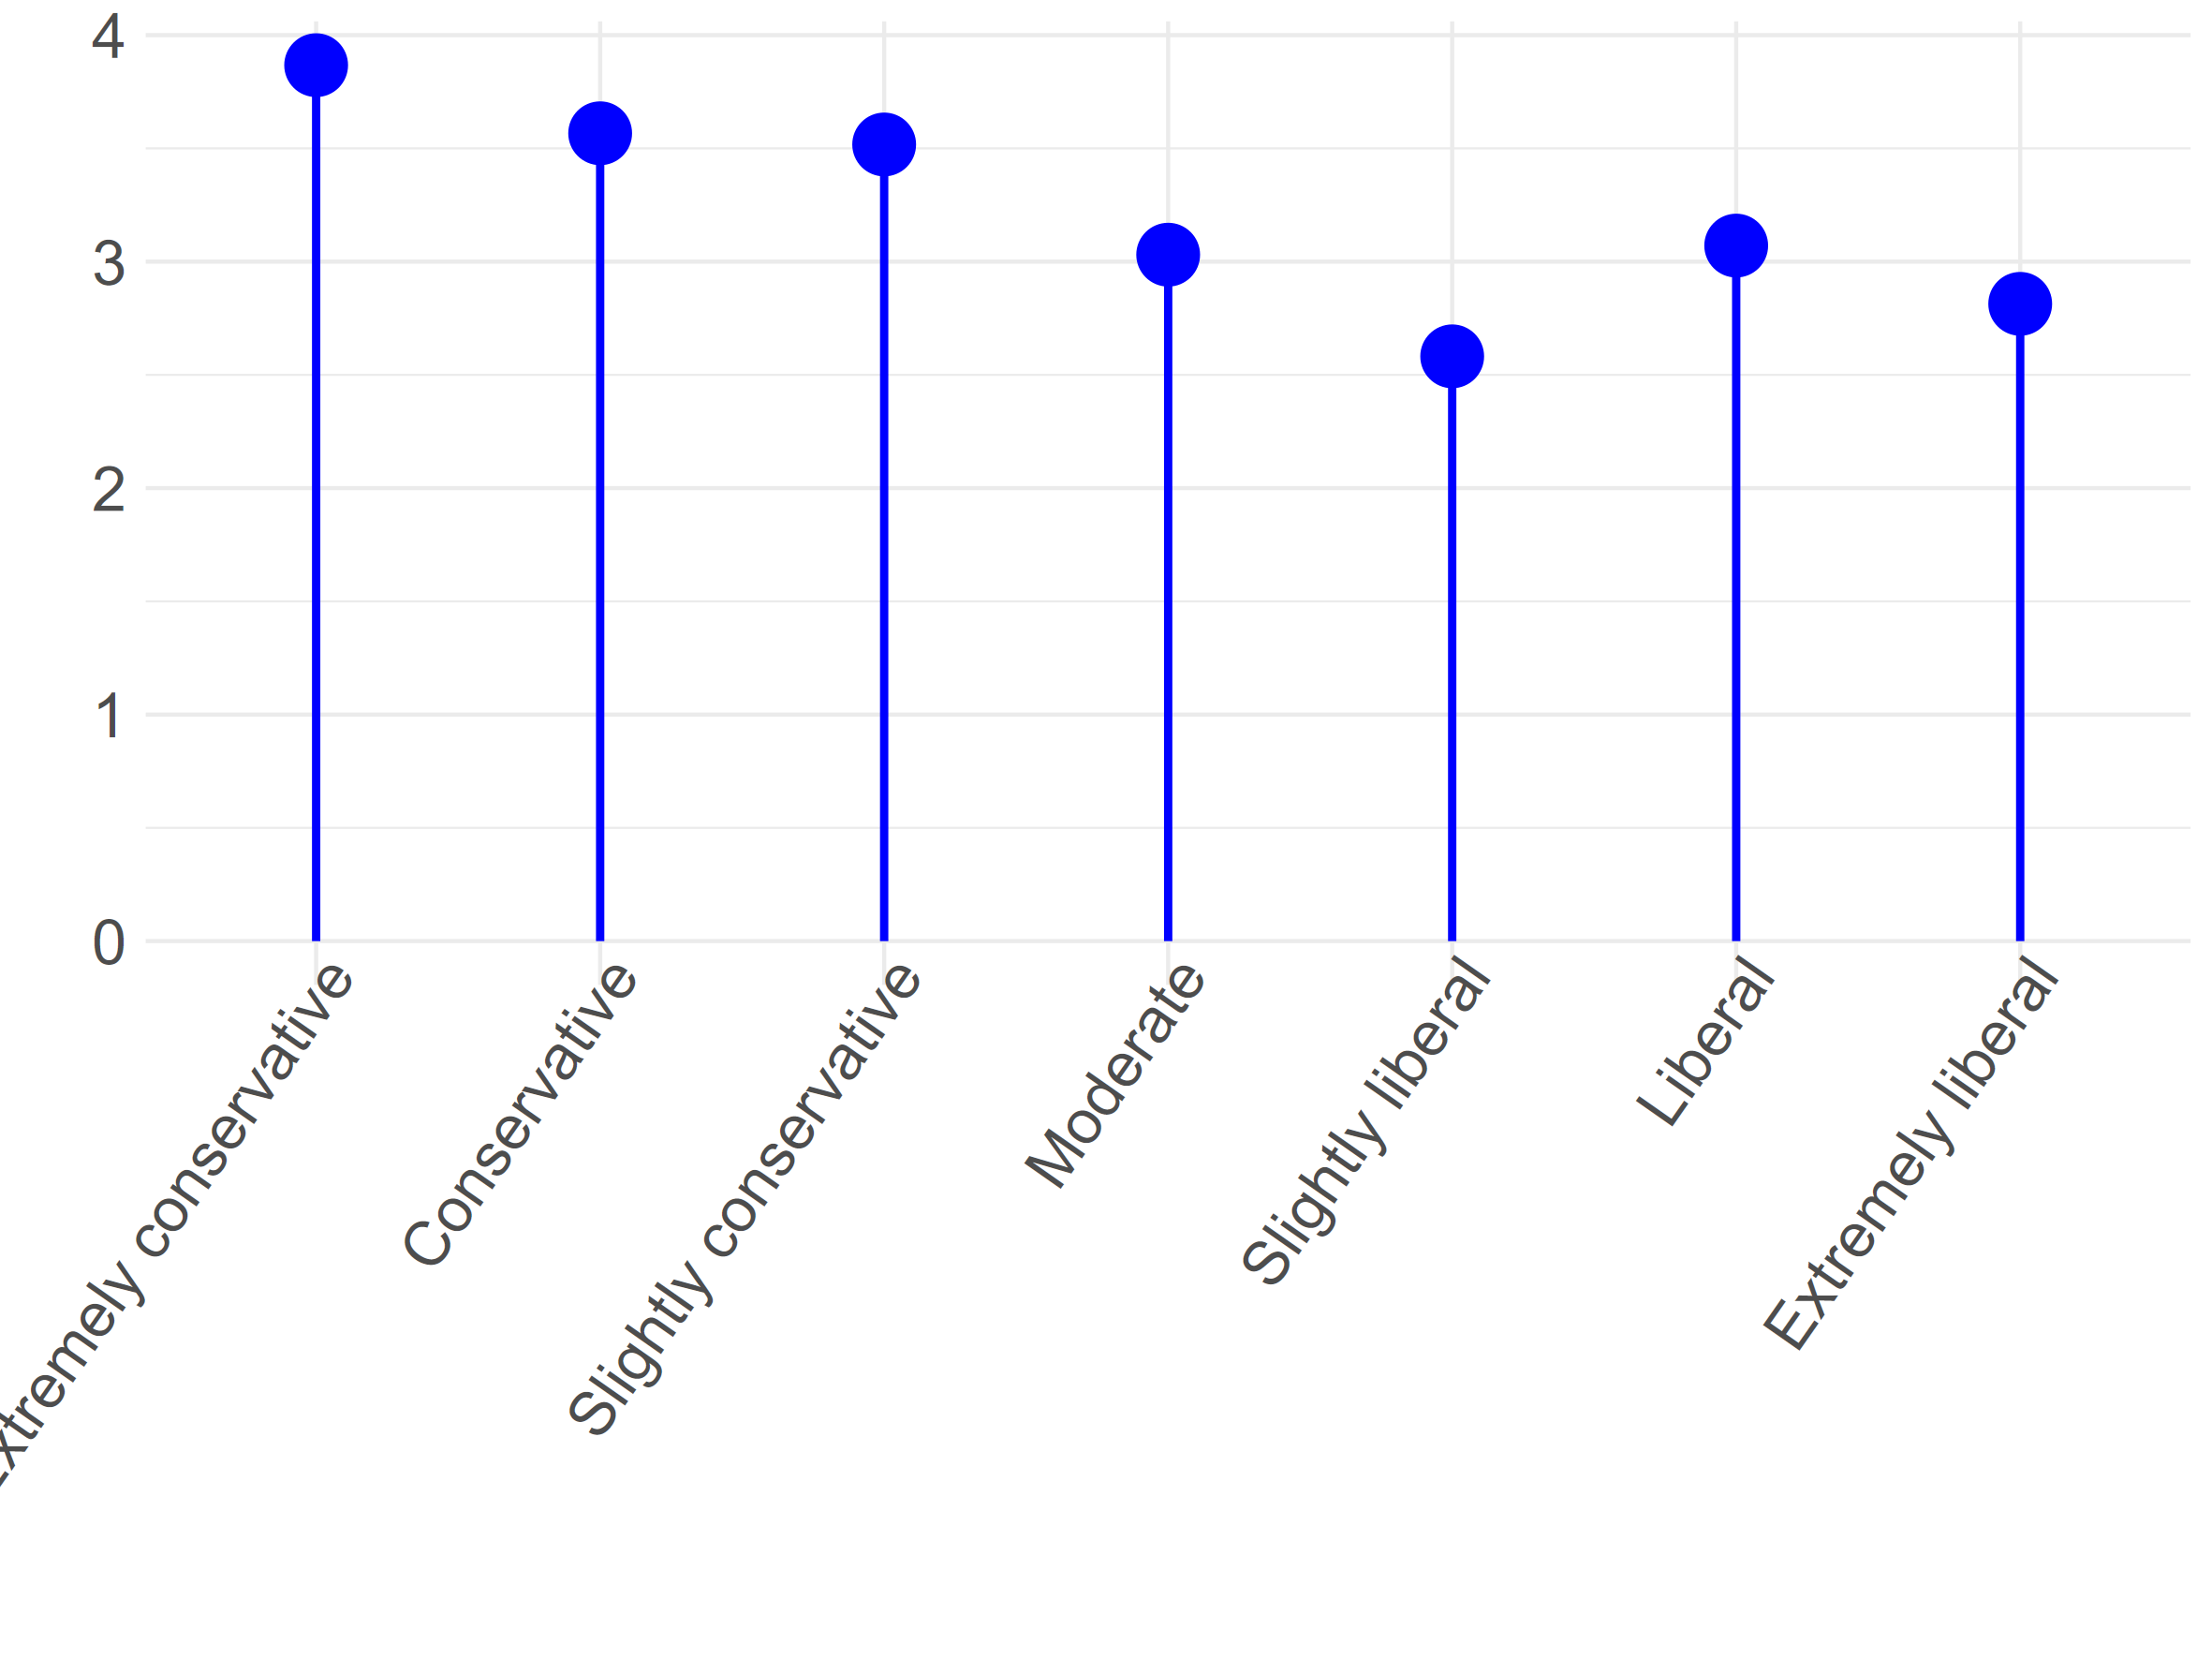
\includegraphics[width=1.0\textwidth]{Plots/uni-dist-grd-int-pol.png}
            \caption{Political Ideology}
            \label{fig:grd-int-pol}
    \end{subfigure}
     \begin{subfigure}[b]{0.3\textwidth}
        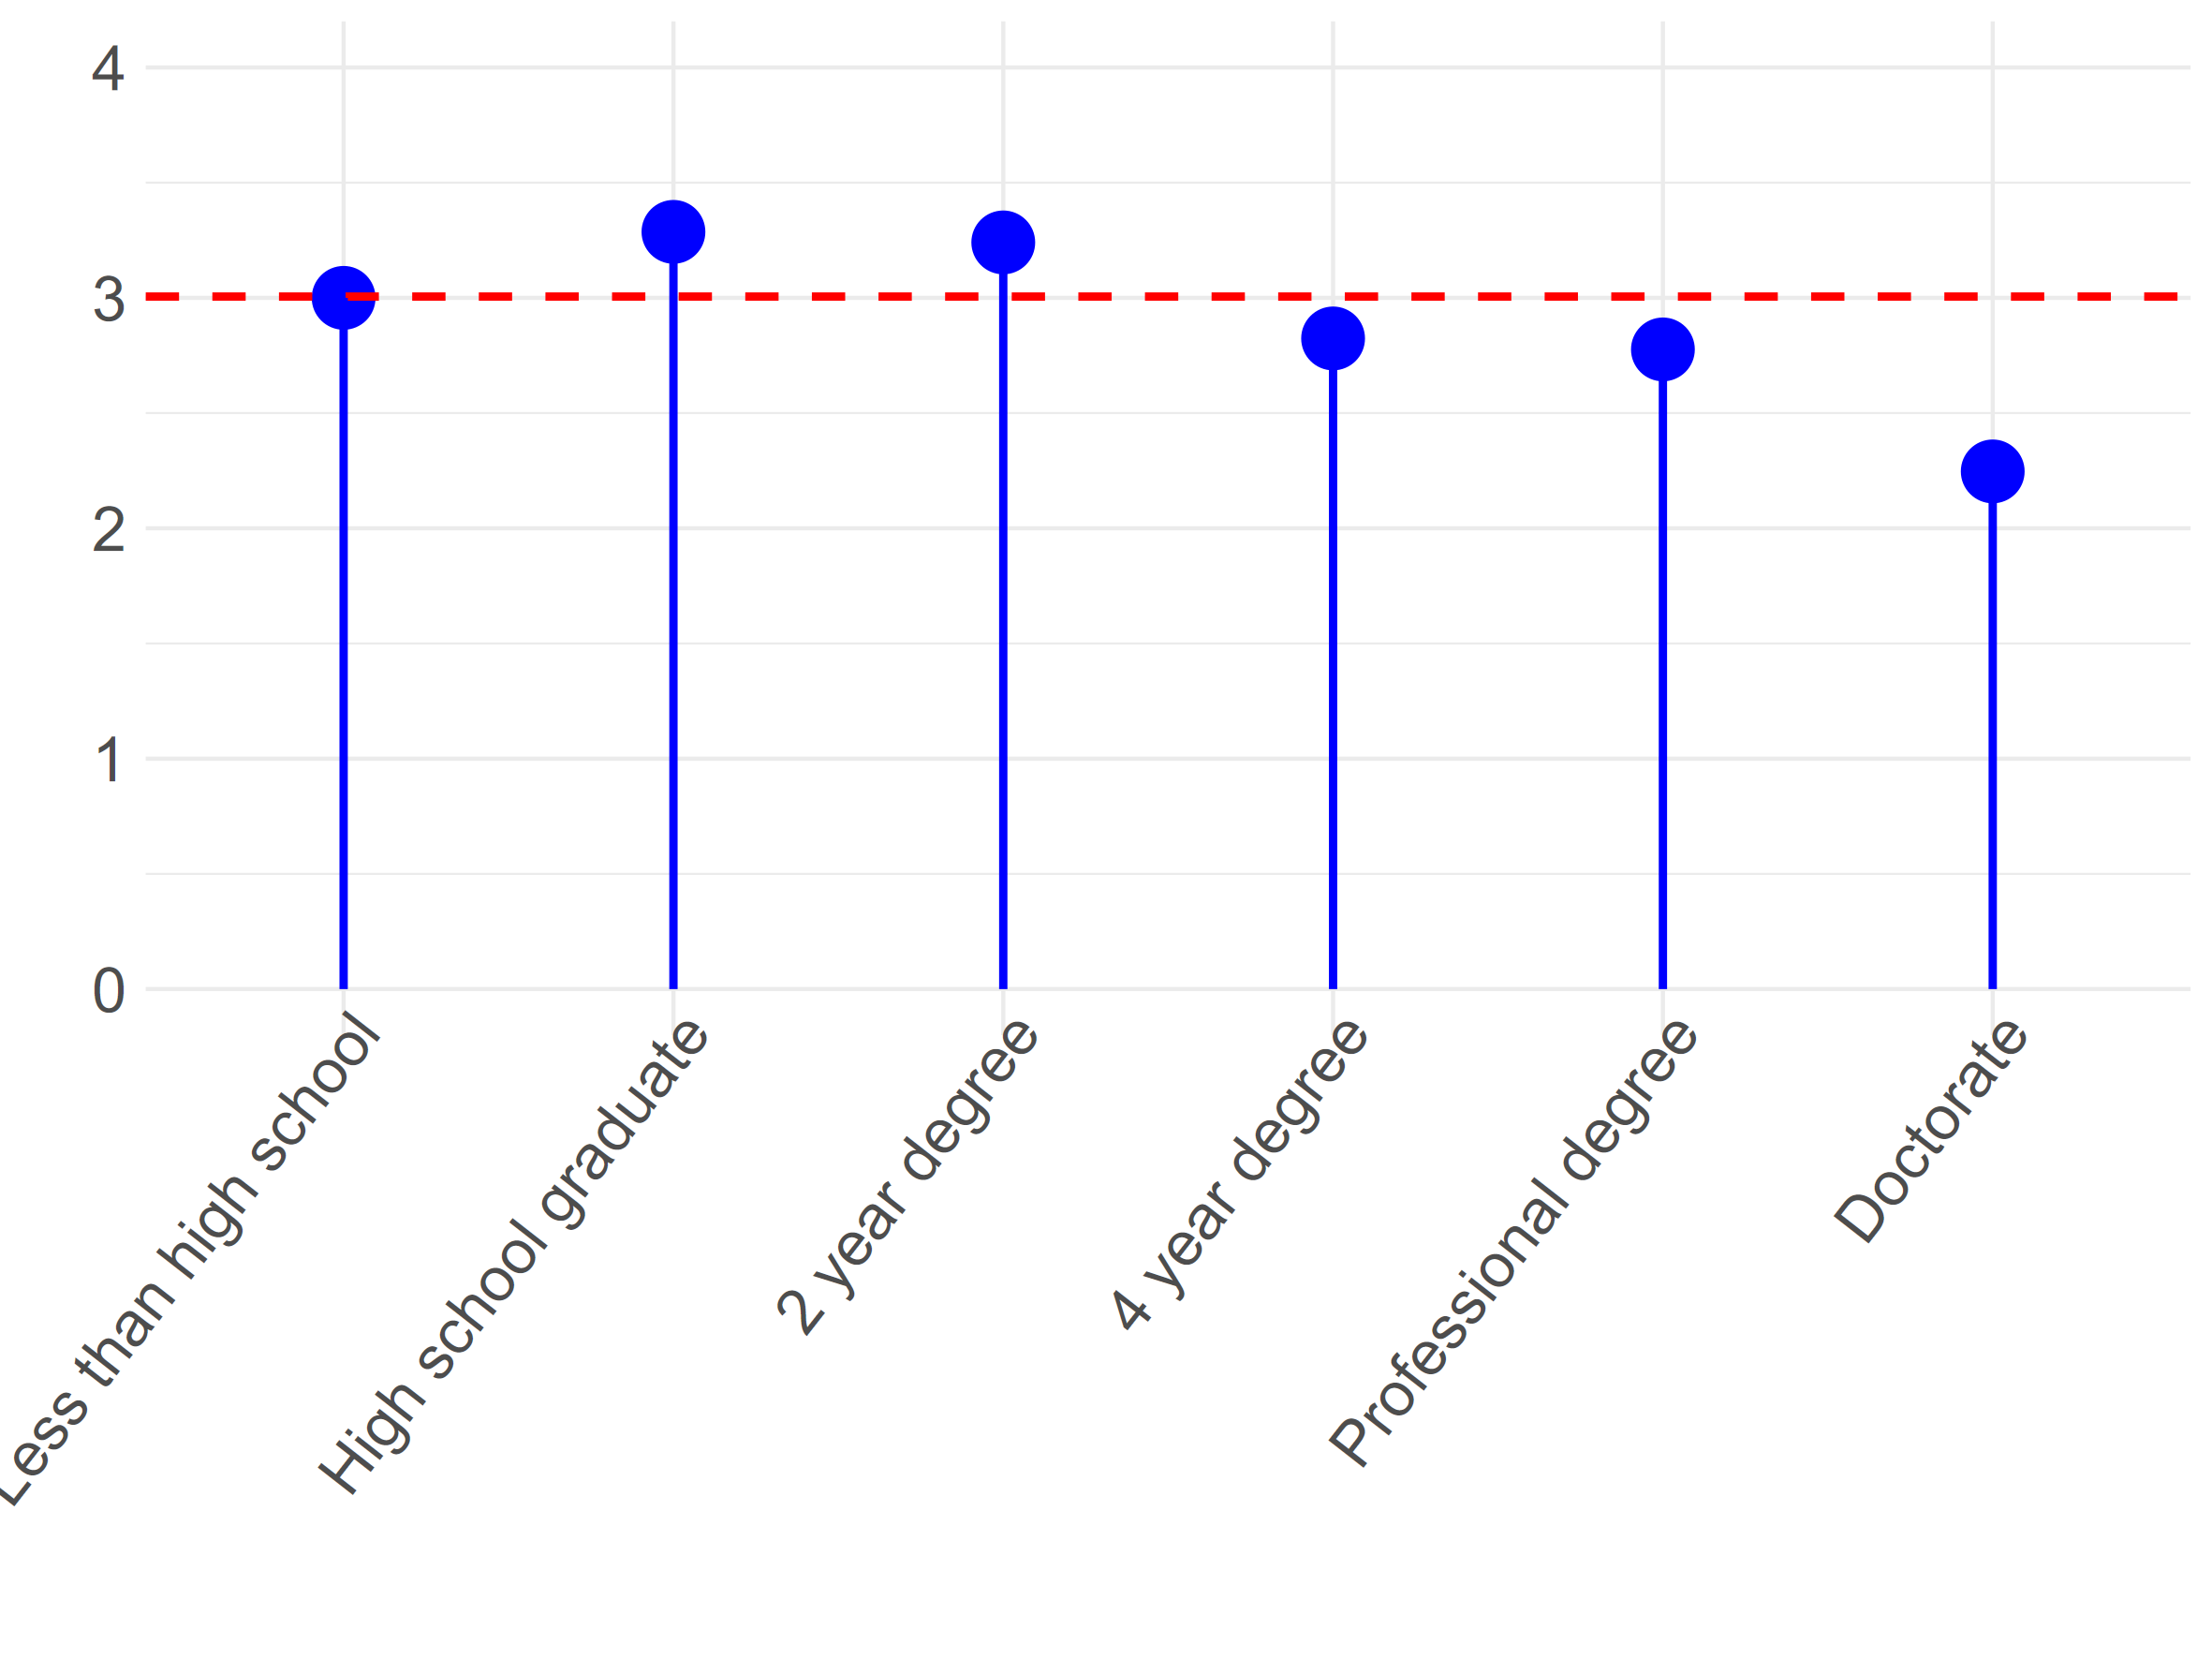
\includegraphics[width=1.0\textwidth]{Plots/uni-dist-grd-int-edu.png}
            \caption{Education}
            \label{fig:grd-int-edu}
    \end{subfigure}
     \begin{subfigure}[b]{0.3\textwidth}
        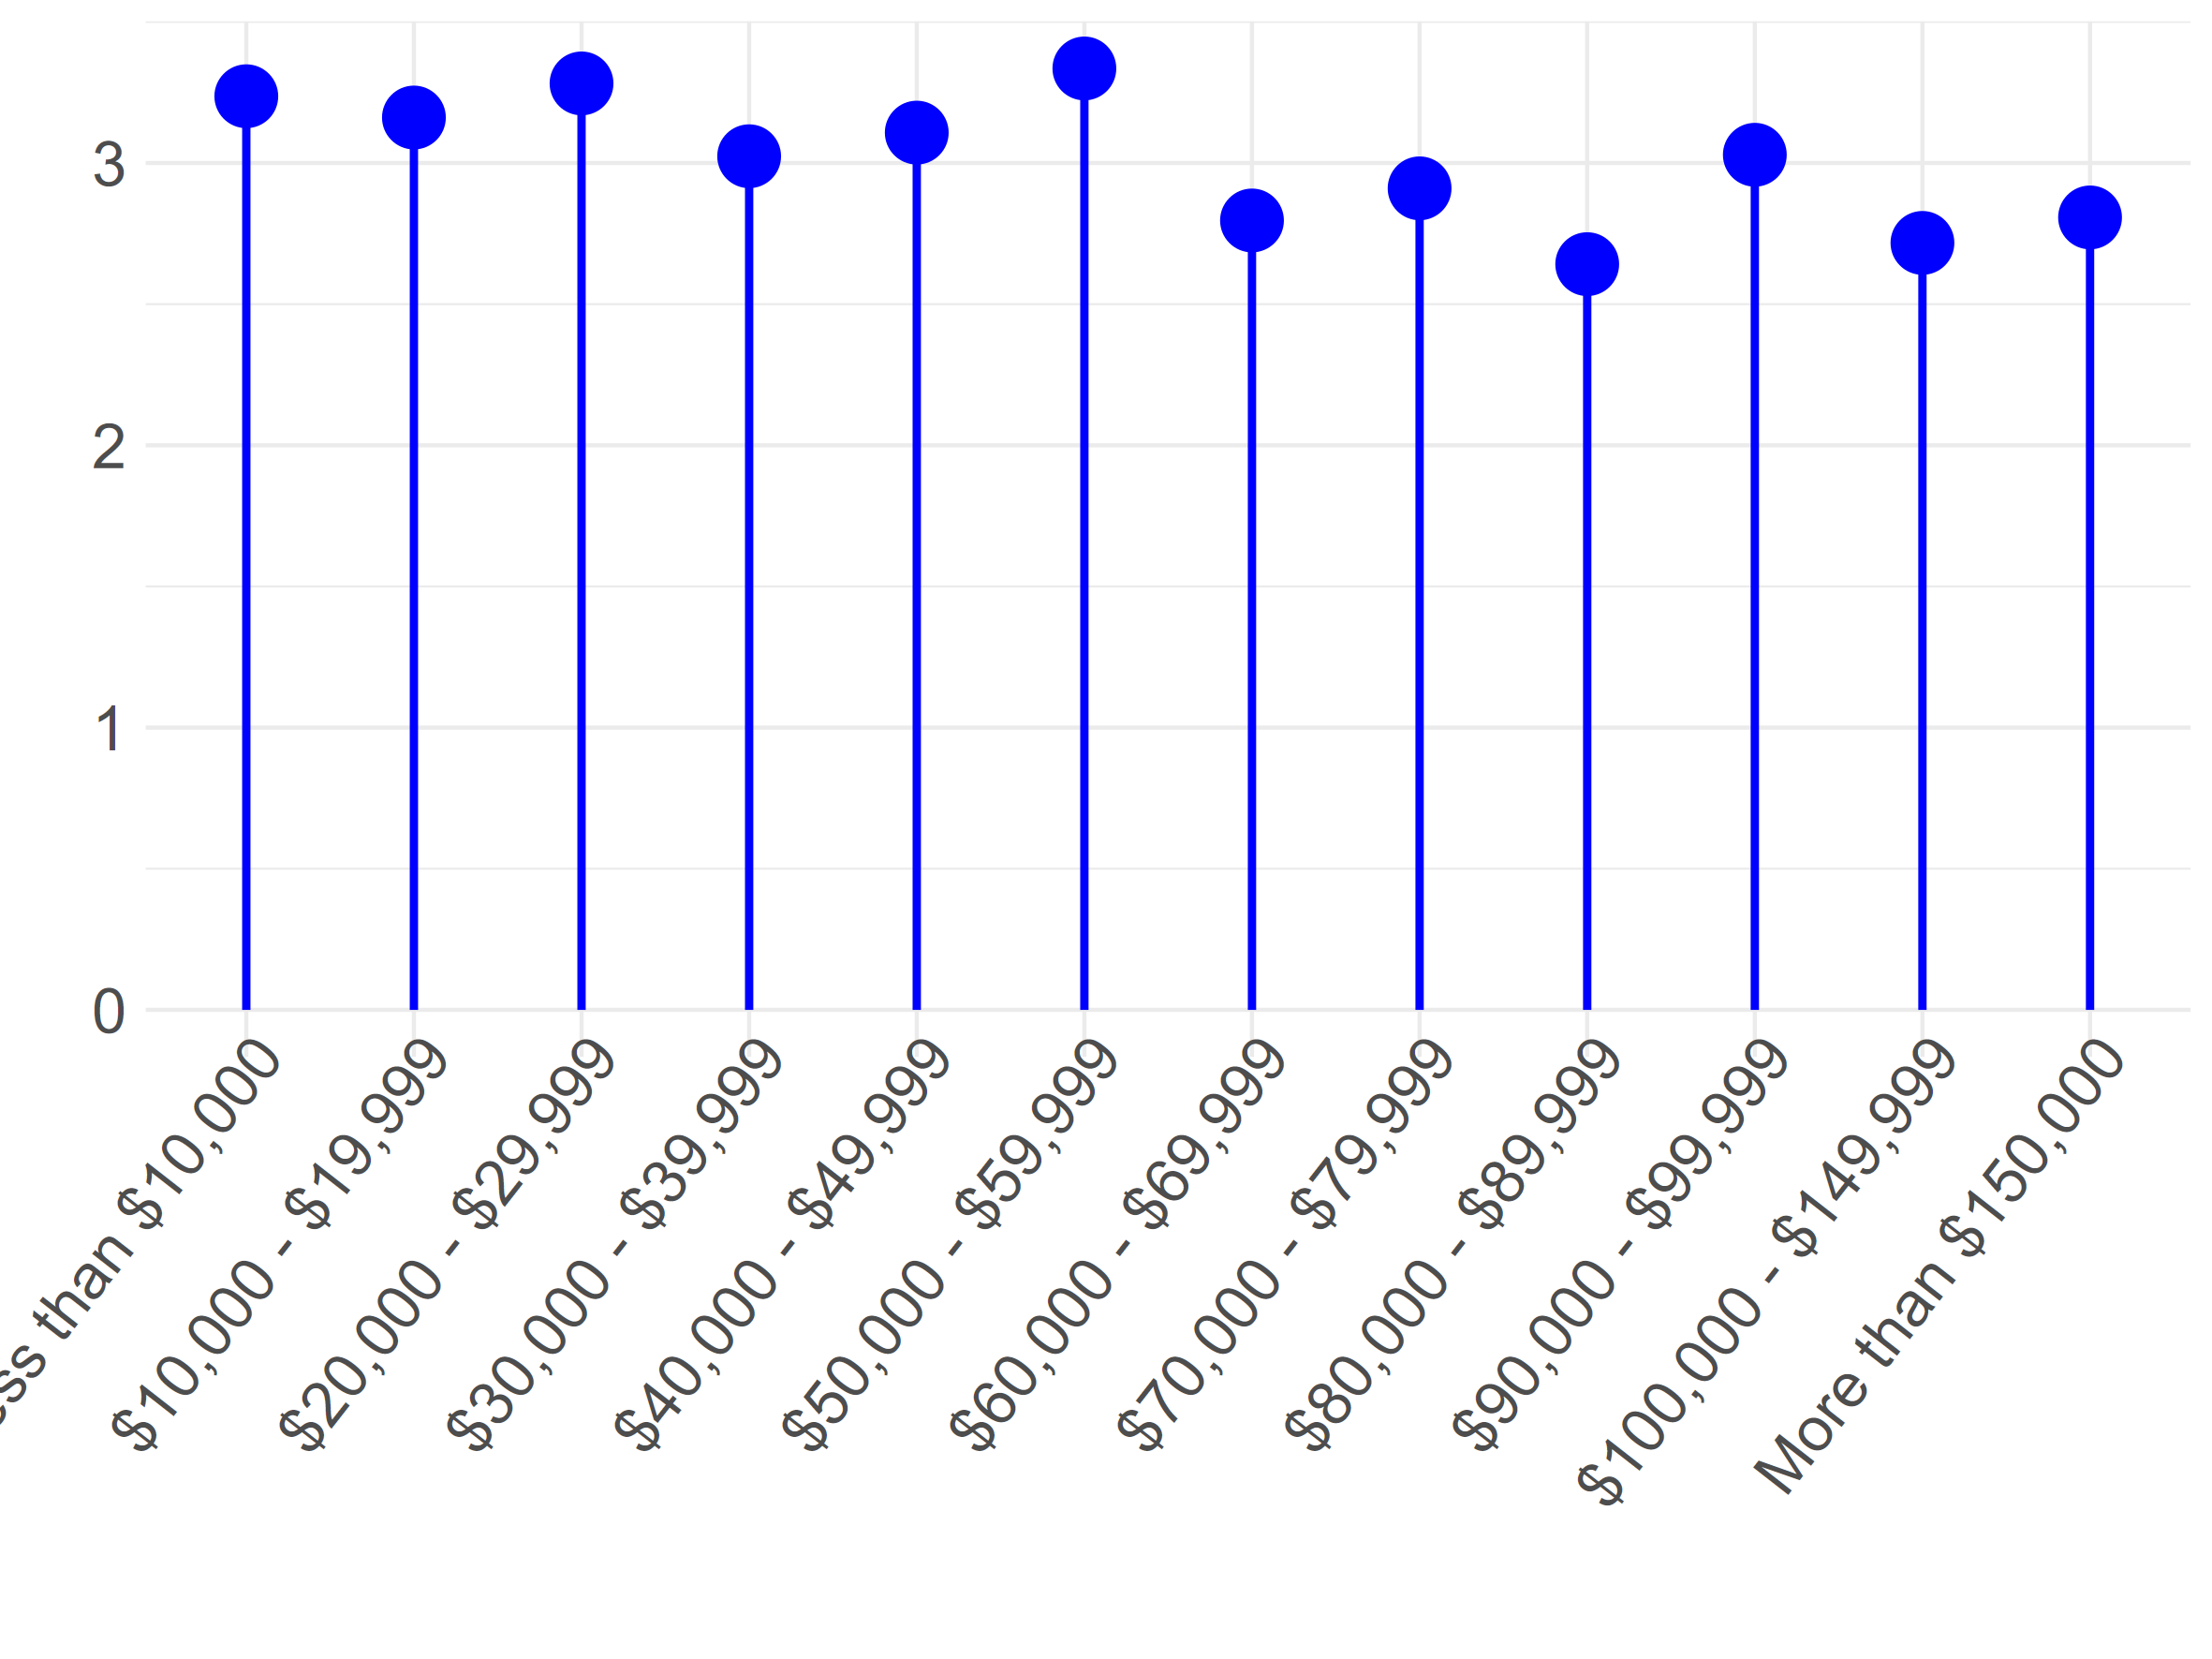
\includegraphics[width=1.0\textwidth]{Plots/uni-dist-grd-int-inc.png}
            \caption{Income}
            \label{fig:grd-int-inc}
    \end{subfigure}
     \begin{subfigure}[b]{0.3\textwidth}
        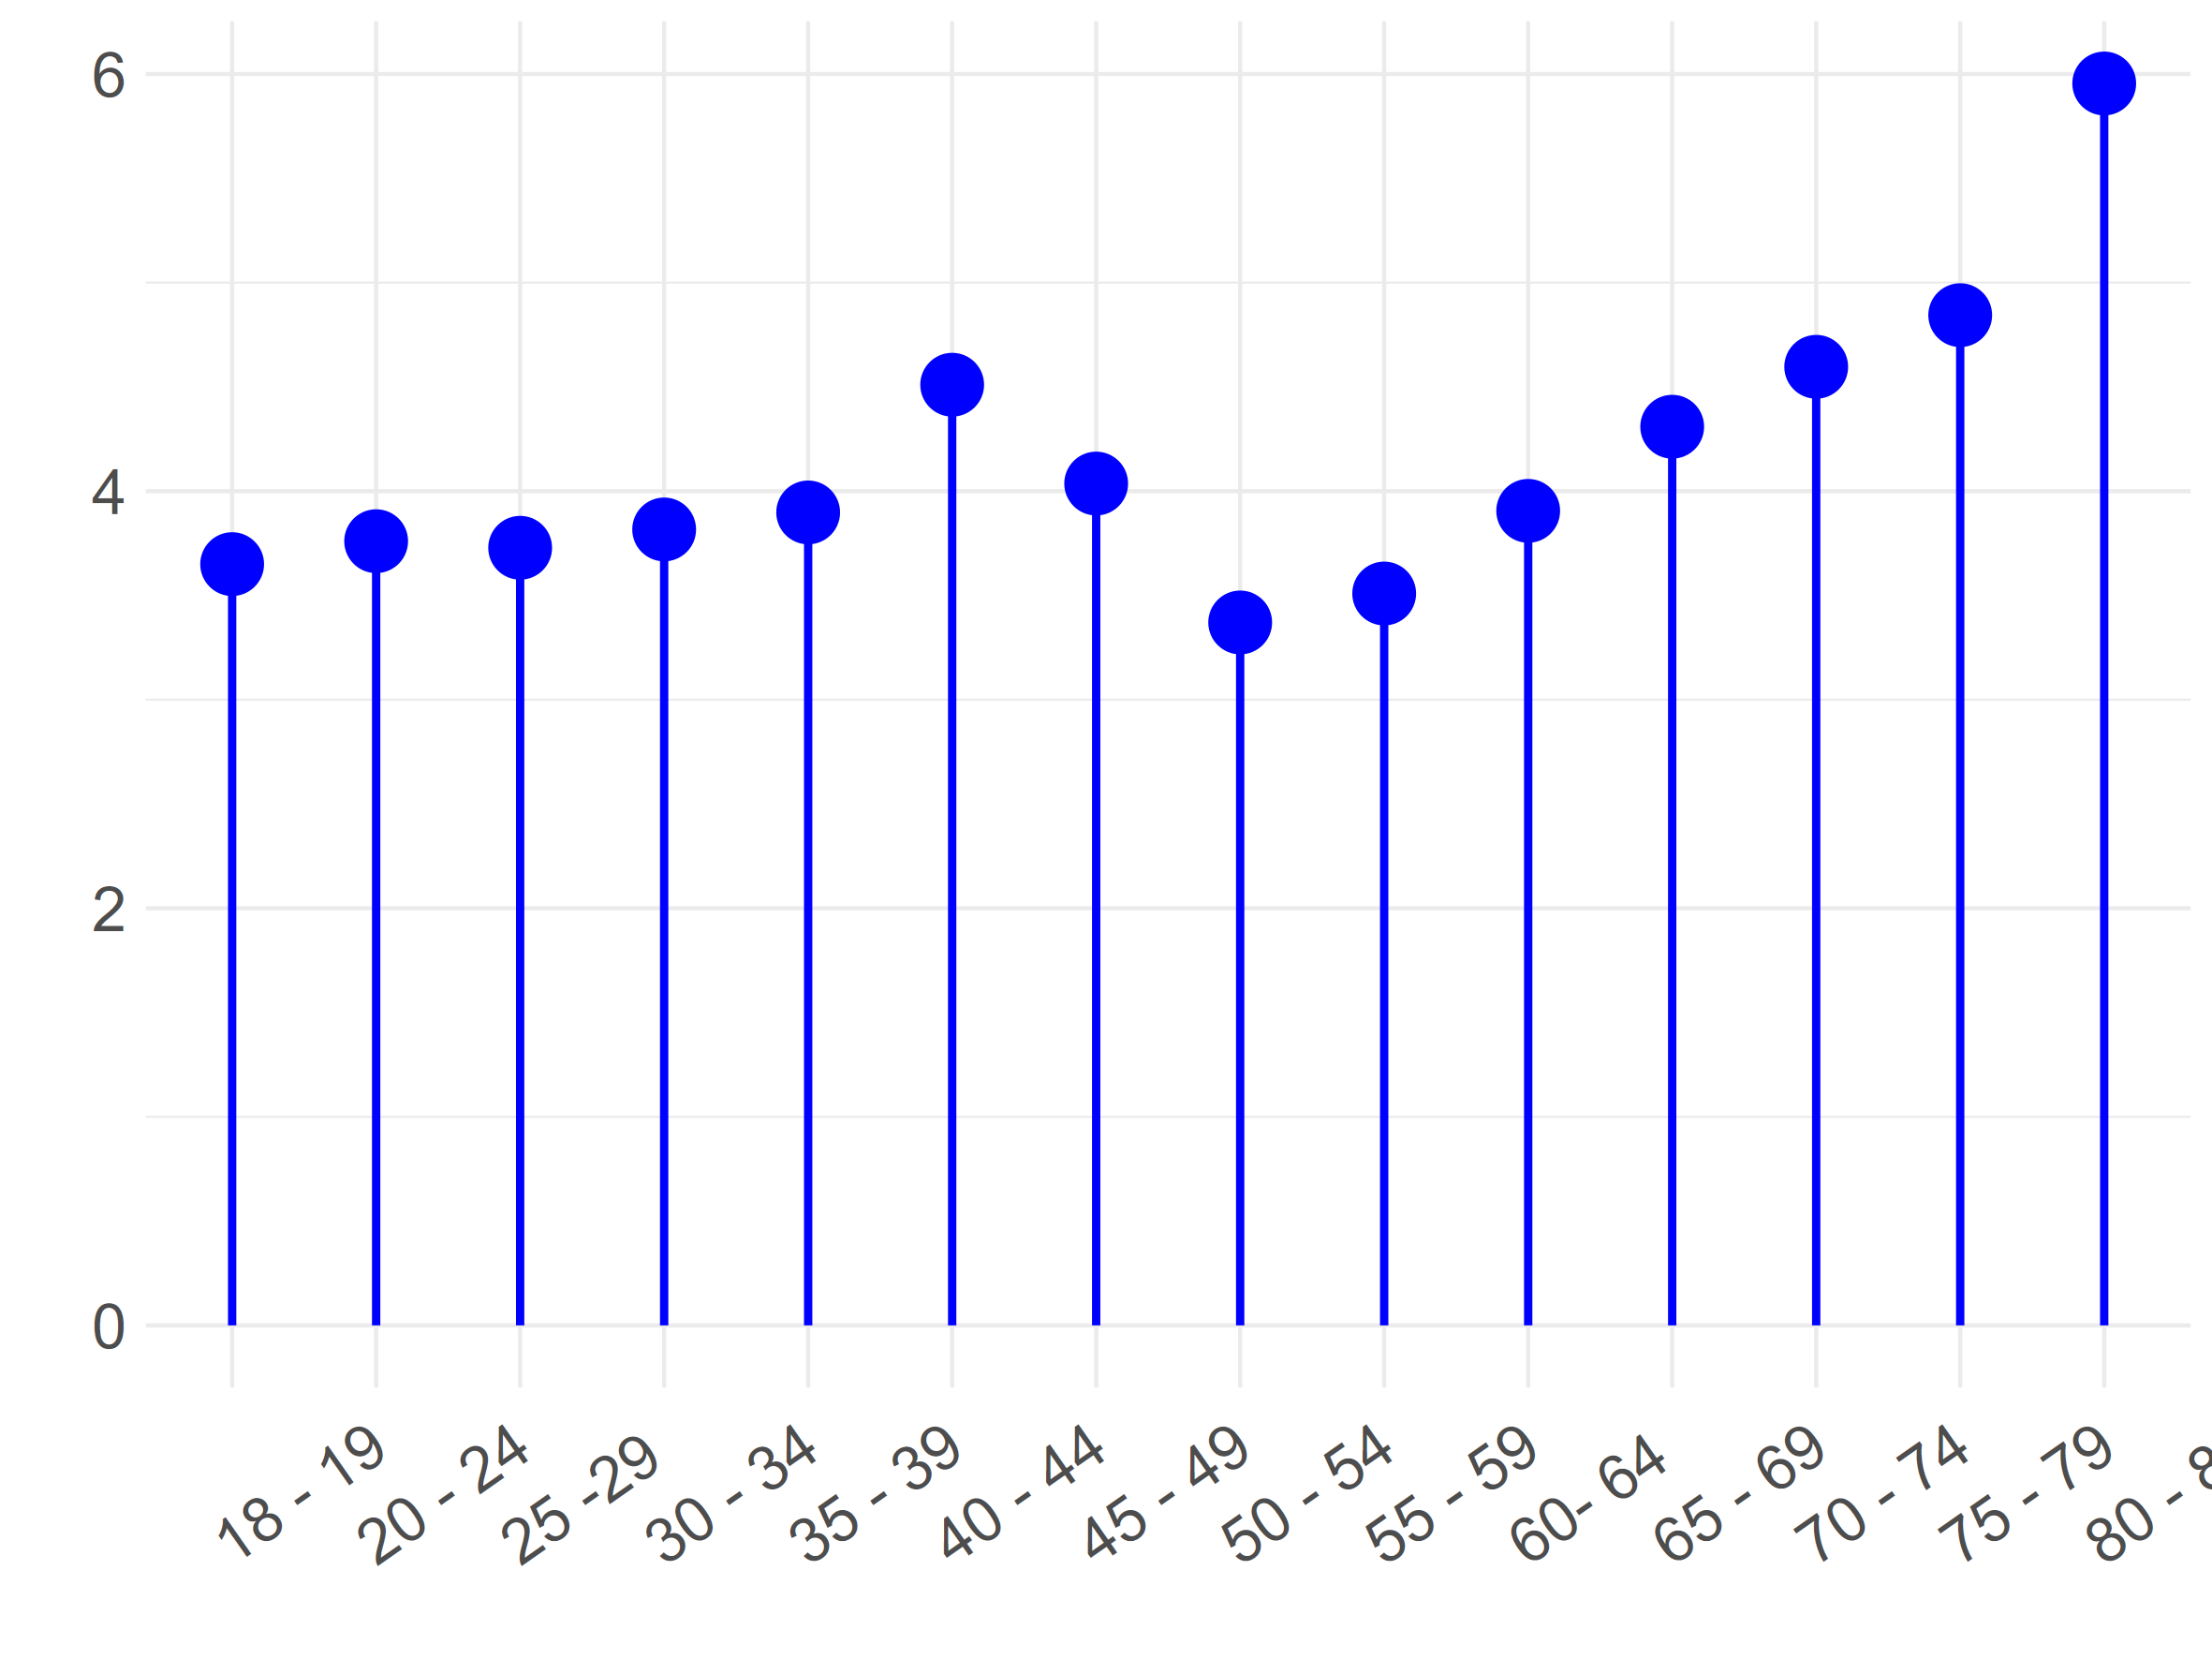
\includegraphics[width=1.0\textwidth]{Plots/uni-dist-grd-int-age.png}
            \caption{Age}
            \label{fig:grd-int-age}
    \end{subfigure}
     \begin{subfigure}[b]{0.3\textwidth}
        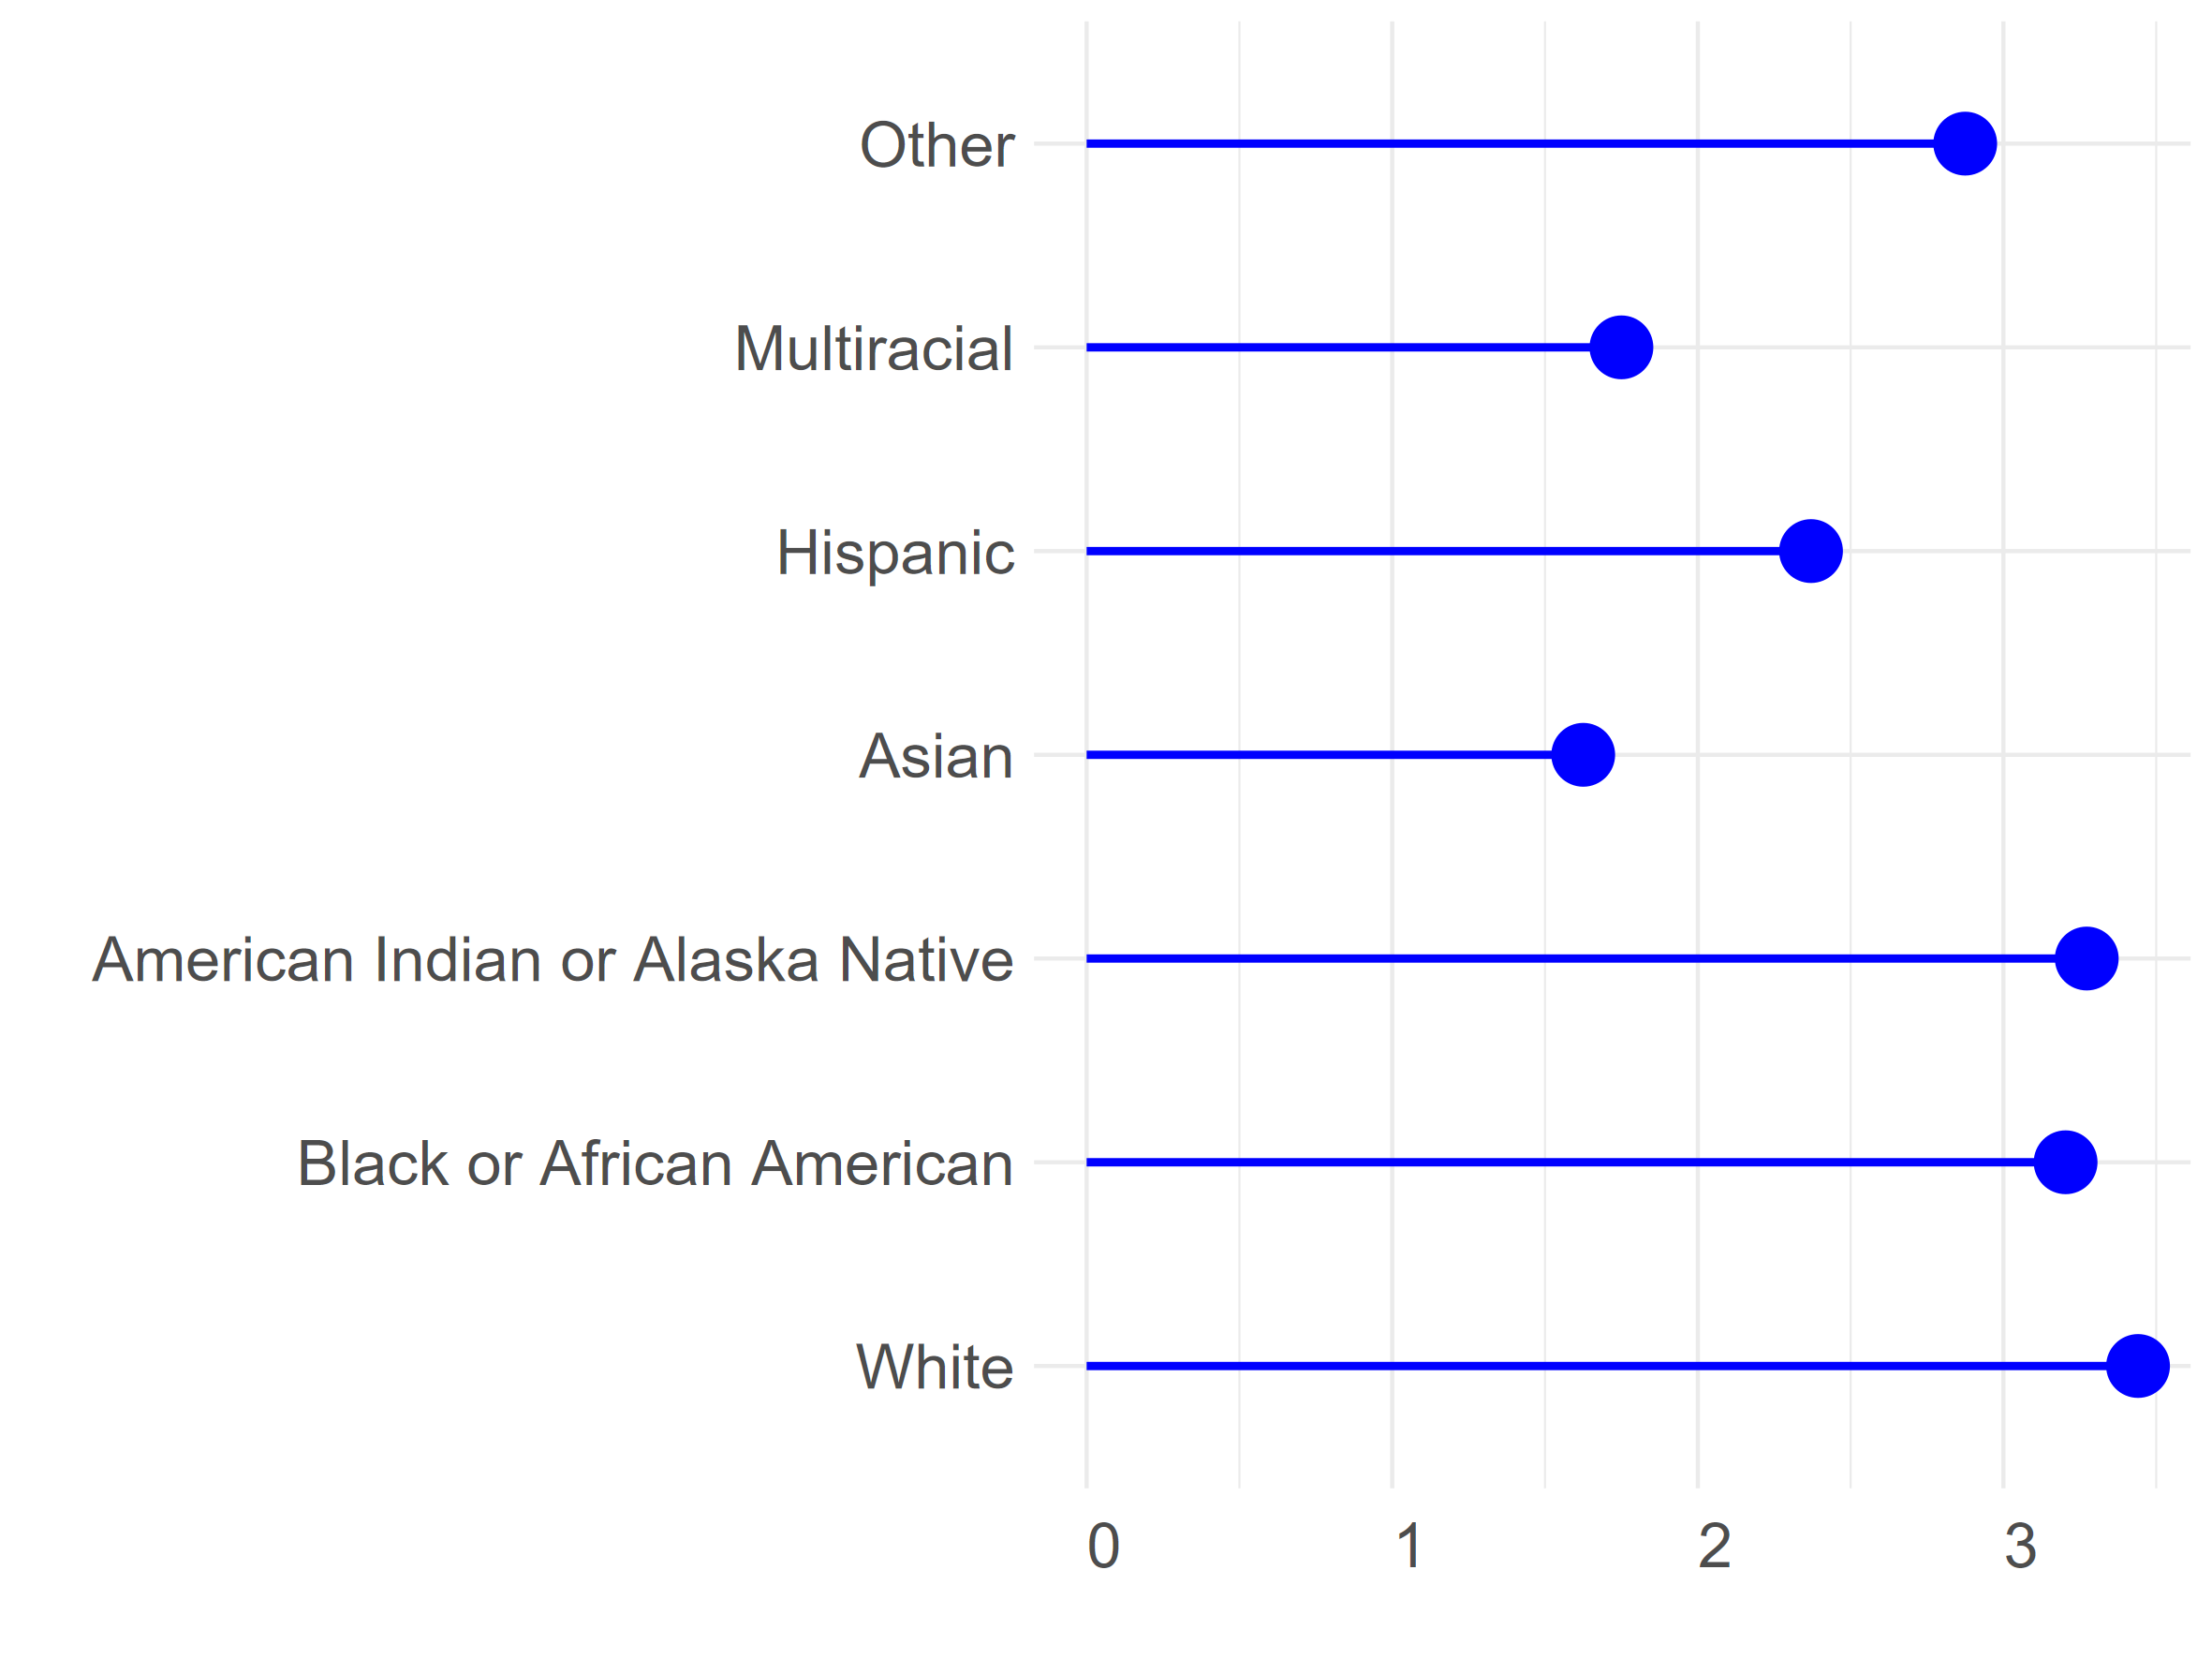
\includegraphics[width=1.0\textwidth]{Plots/uni-dist-grd-int-rac.png}
            \caption{Ethnoracial Identification}
            \label{fig:grd-int-rac}
    \end{subfigure}
     \begin{subfigure}[b]{0.3\textwidth}
        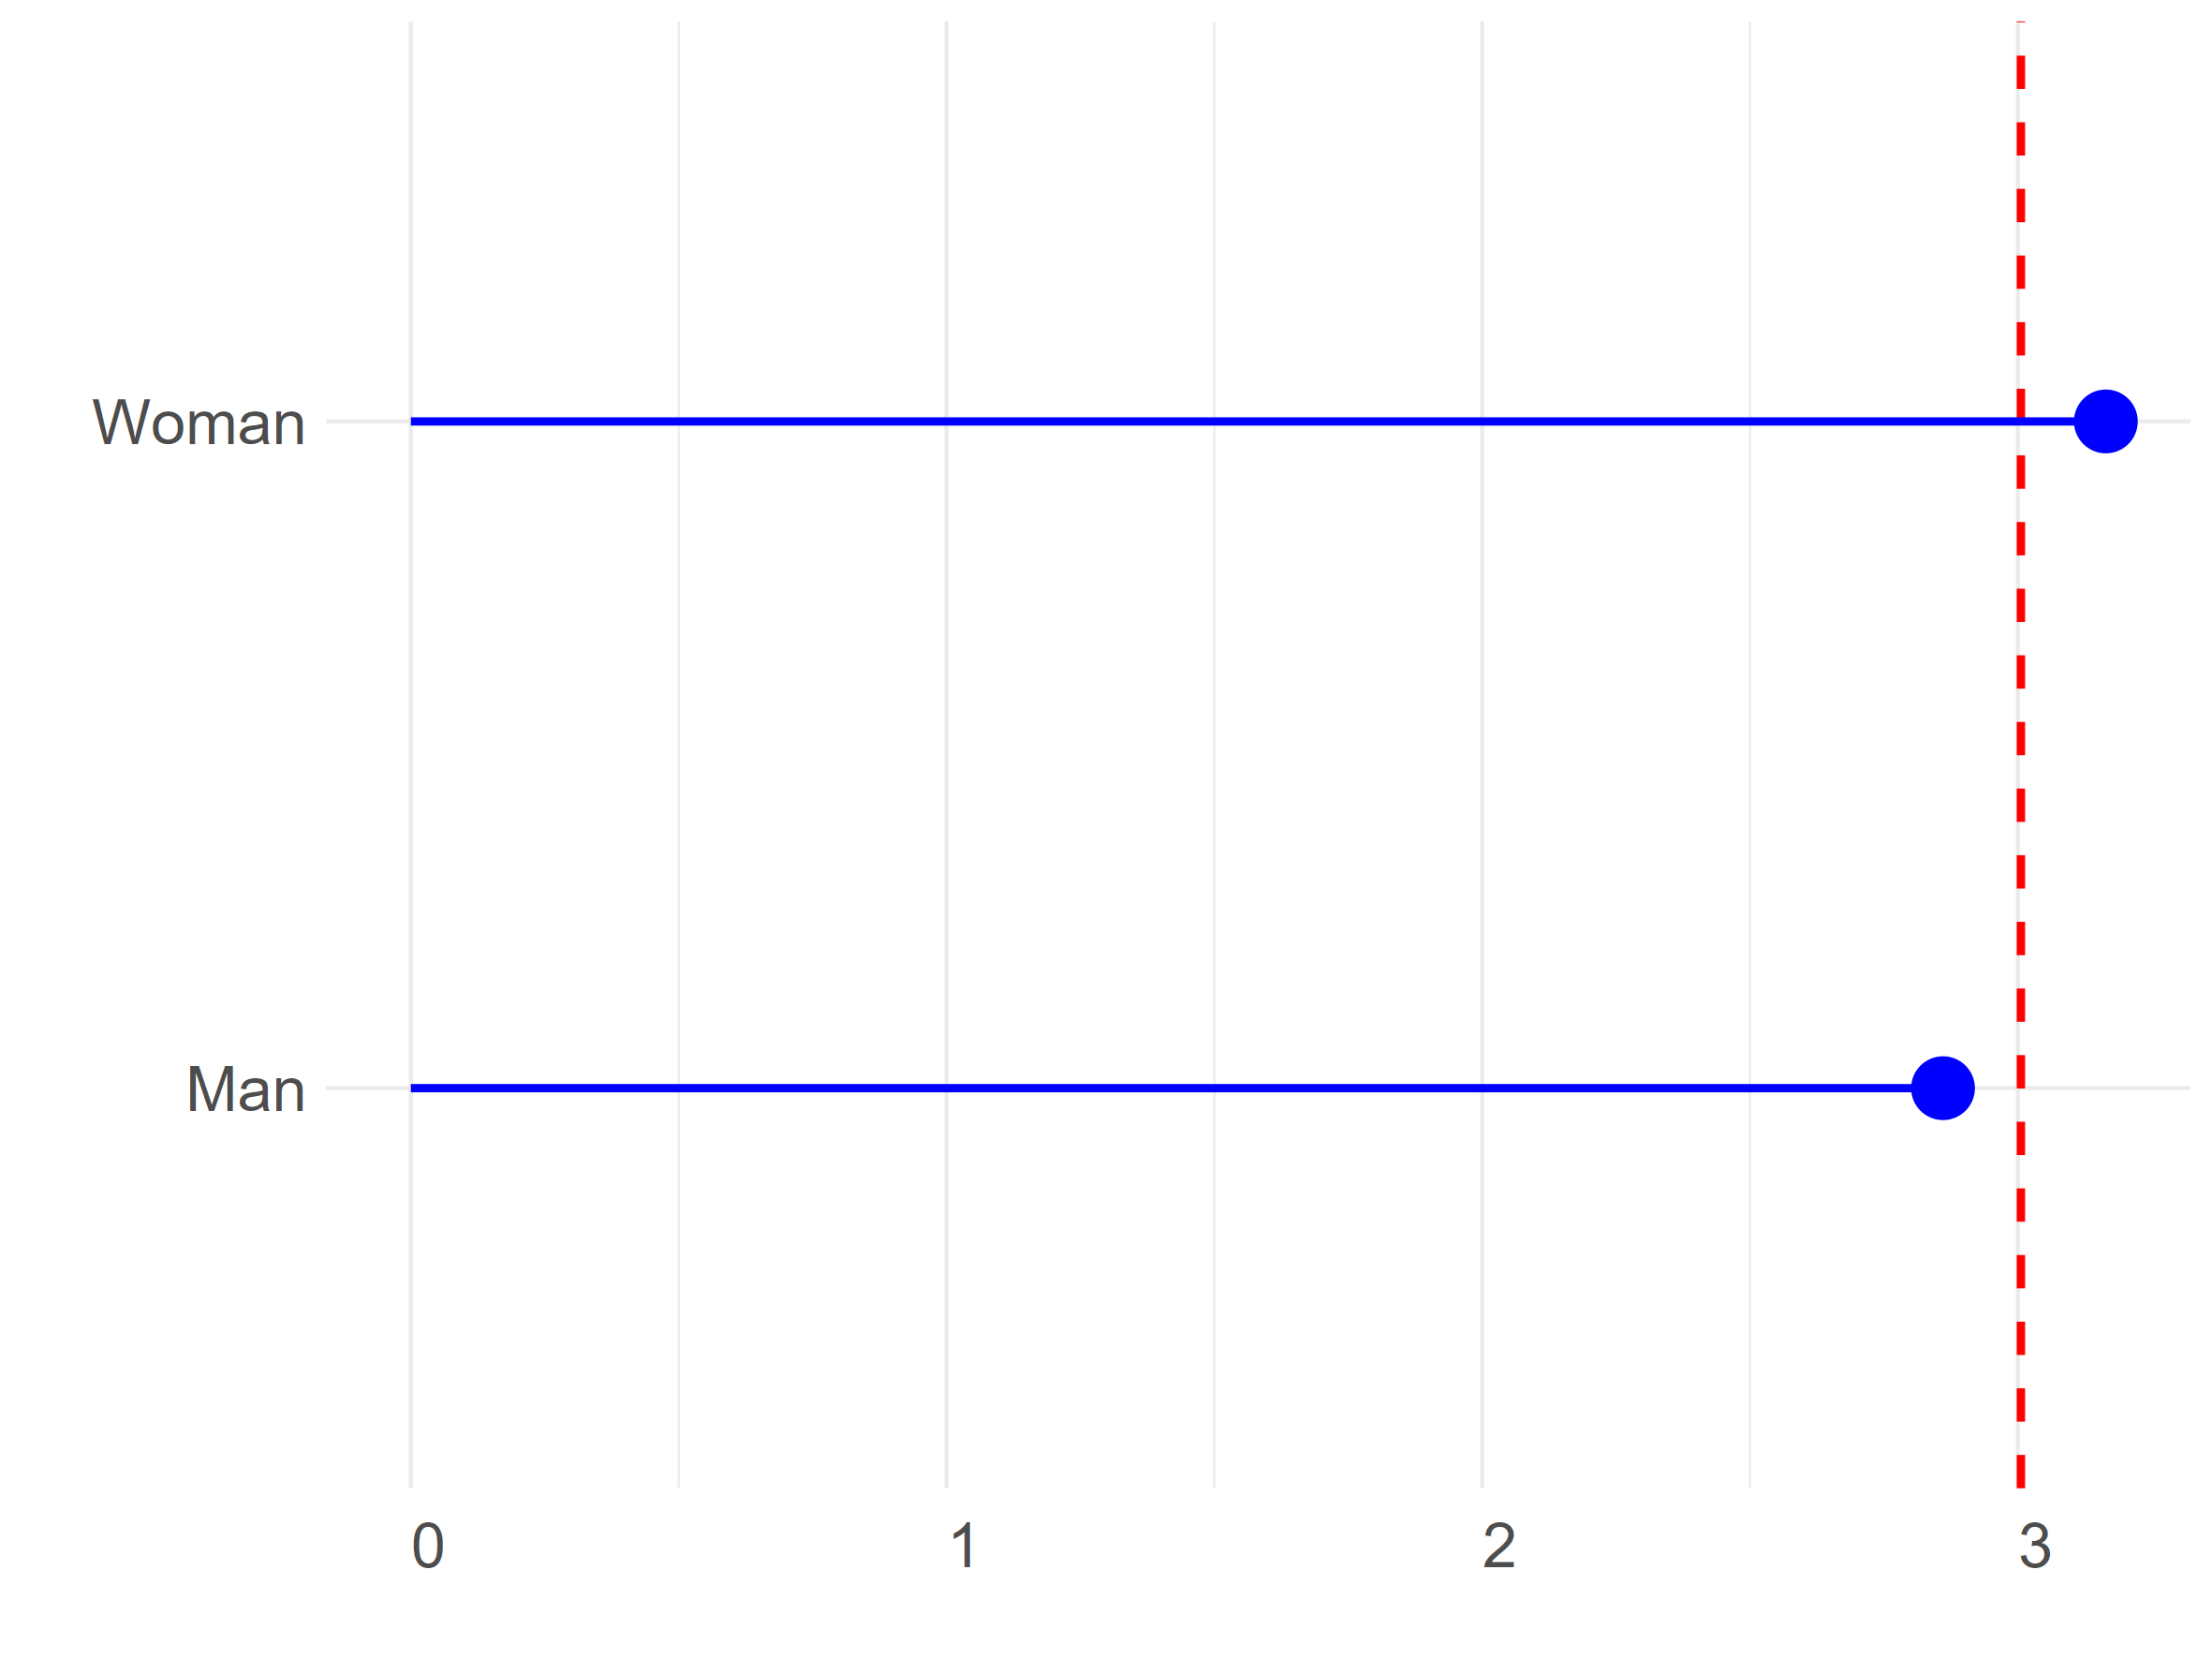
\includegraphics[width=1.0\textwidth]{Plots/uni-dist-grd-int-gen.png}
            \caption{Gender Identification}
            \label{fig:grd-int-gen}
    \end{subfigure}
    \caption{Average number of cultural dislikes across different socio-demographic characteristics.}
    \label{fig:grd-int}
\end{figure}

Symbolic exclusion propensities among different groups can be straightforwardly accounted for by age and education, with older, less educated respondents expressing more dislikes than younger, more educated ones. Importantly, symbolic exclusion is also structured by political ideology in the expected direction---see \citet{rawlings2023polarization-0af}---with liberals being less likely to express cultural dislikes than self-identified conservatives. In the same way, non-whites in the sample are less likely to express cultural dislikes (compared to white respondents), while women express more dislikes (compared to those who identify as men). 

\section*{Zero-Inflated Poisson Regression Models}
In their original paper, \citet{lizardo2016end-4fb} proposed modeling categorical tolerance and symbolic exclusion jointly as a hurdle process. The basic idea is that categorical tolerants are a distinct slice of the population who are not at risk of engaging in symbolic exclusion (expressing dislikes). Thus, we can statistically model the joint predictors of both tendencies by assuming that there is a set of predictors that drive the probability of being in the categorical tolerant group (thus not being at risk of expressing dislikes), and net of this, there is a second set of predictors that drive the number of dislikes expressed for those who are at risk of doing so. The zero-inflated Poisson model is thus a natural framework for modeling this dual regime data-generating process \citep{zorn1998analytic-6b1}. 

\begin{table}
    \caption{Coefficient Estimates from Zero-Inflated Poisson Models Predicting Categorical Tolerance and Symbolic Exclusion, Joint Prolific and Lucid Samples.}
    \centering
    
\includegraphics[trim={0 0 0 0},clip, width=1.0\textwidth]{Tabs/zinf-reg.png}
    \label{tab:zinf}
\end{table}

Table~\ref{tab:zinf} shows the coefficient estimates from a set of four zero-inflated Poisson regression models. The specifications in each model, for both the count and zero-inflated components, are informed by the descriptive patterns we considered in Figures~\ref{fig:cat-tol} and~\ref{fig:grd-int}. Coefficient estimates corresponding to the count part of the model---predicting the number of dislikes among those who are at risk of expressing them---are shown in the top half of the table. Coefficient estimates for the zero-inflation part of the model, predicting the odds of landing in the categorical tolerant group---and thus not being at risk of engaging in symbolic exclusion---are presented in the lower half of the table. In all models, age, education, income, and political ideology (with higher values indicating a more liberal stance) are entered as ordered numerical inputs. Race (White) and Gender (Female) are entered into the model as dummy indicators. The zero-inflated specifications also contain squared terms for education and income to model expected curvilinear effects (see Figures~\ref{fig:cat-tol-edu} and~\ref{fig:cat-tol-inc}).

Let us begin with the predictors of symbolic exclusion; 

\newpage
\bibliography{references}
\bibliographystyle{apalike}

\end{document}
